% Chapter 1

\chapter{Numerical Simulation of Solidification Process} % Main chapter title

\label{Chapter3} % For referencing the chapter elsewhere, use \ref{Chapter1} 
\section{OpenFOAM. General Aspects}

\setlength{\parindent}{0.5cm} OpenFOAM is a free open-source software written in C++ and mainly conceived to perform computational fluid dynamics (CFD) simulations based on a finite volume discretization (FVM). 

\subsection{The finite volume method}

\setlength{\parindent}{0.5cm} Fluid equations usually take the form of non-linear partial differential equations and so, most of time, no analytical solution can be derived from them. In that context, different numerical techniques are employed to reach an approximation of the solution to these problems. These methods require a discretization of the domain in which the solution is going to be calculated. As aforementioned, OpenFOAM uses the finite volume method, which is, indeed, one of the most widely techniques used in computational fluid dynamics, and the one used in this thesis.

\noindent This technique turns the partial differential equations, which at their turn represent conservation laws over differential volumes, into discrete algebraic equations over finite volumes. Similarly to the finite element method, the FVM also needs a discretization of the geometric domain but in this numerical method, the elements used to integrate the algebraic equations representing the conservation partial differential equations are finite volumes.

\noindent Some of the terms in the conservation equation are converted into face fluxes and evaluated in the discretized finite volumes. These face fluxes are strictly conservative. This is that the flux entering the volume is equal to the flux leaving the adjacent volume. This property makes the finite volume method the preferred technique for CFD \cite{moukalled_mangani_darwish_2016}. 

\subsubsection*{Geometric domain discretization}

\setlength{\parindent}{0.5cm} The intrinsic properties of the finite volume method need the computational domain to be discretized in volume cells, known as control volumes (CV). Each one of these volumes has a centroid or computational point in which the solution is obtained. 

\noindent Alongside with this idea, OpenFOAM follows a cell-centered approach in which the unknowns are defined at the center of these volumes or cells. The value of these are computed as an average value of the variable in that cell.

\noindent Moreover, the control volume is defined by the neighbours. This is, in the case the volume has an adjacent neighbour, an internal face is delimiting the separation of both. On the other hand, if the volume is not sharing a face with a neighour volume, the face is considered to be a boundary.

\subsubsection*{Discretization of the fluid dynamic's equations}

\setlength{\parindent}{0.5cm} The continuity equation, the Navier-Stokes equations and, the heat equation stated in section 2 can be stated in a more general form under the formulation of the Reynolds transport theorem:
\begin{equation}
	\underbrace{\int_{V_{P}} \frac{\partial \rho \phi}{\partial t} d V}_{\text {Temporal term }}+\underbrace{\int_{V_{P}} \nabla \cdot(\rho \vec{u} \phi) d V}_{\text {Convective term }}=\underbrace{\int_{V_{P}} \nabla \cdot\left(\rho \Gamma_{\phi} \nabla \phi\right) d V}_{\text {Diffusive term }}+\underbrace{\int_{V_{P}} S_{\phi} d V}_{\text {Source term }}
	\label{3.1}
\end{equation}
where $V_{P}$ is the control volume cell, $\phi$ may be any scalar or vectorial variable of the continuum, $\Gamma_{\phi}$ is the diffusivity of the variable and $S_{\phi}$ is a source term. 

\noindent In order to recover the continuity, momentum and energy equations, the parameters shown in table \ref{3.1tab} need to be shaped in the transport equation.
\begin{table}[h!]
	\begin{tabular}{@{}lllll@{}}
		\toprule[1pt]
		\textbf{Equation} & \textbf{$\phi$} & \textbf{$\Gamma_{\phi}$} & \textbf{$S_{\phi}$}  \\ \midrule[2pt]
		\textbf{Continuity} & 1 & 0 & 0  \\
		\textbf{Momentum} & $\vec{u}u$ & $\nu$ & -$\nabla p$\\
		\textbf{Energy} & $C_{p}T$ & $\kappa$ & 0\\ \bottomrule[1pt]		
	\end{tabular}
	\centering
	\caption{Parameters to recover continuity, momentum and energy equations.}	
	\label{3.1tab}
\end{table}
\newline
The fluid variable is defined as a ratio of itself integrated along the volume cell. Thus, it yelds the following form,
\begin{equation}
	\phi=\phi_{P}=\frac{1}{V_{p}} \int_{V_{P}} \phi(x) d V
	\label{3.2}
\end{equation}
Therefore, a complete discretization of the previous terms is needed to solve the physics regarding a general fluid dynamics problem.
\subsection{OpenFOAM functioning}
\setlength{\parindent}{0.5cm} In this first section, a brief introduction on the structure and functioning of the OpenFOAM software is given.

\noindent In the folder structure tree shown in Fig. \ref{3.1fig},  it is shown a typical case setup for a phase change problem using \textit{icoReactingMultiphaseFoam} solver.

\begin{figure}[h!]
	\centering
	\scalebox{0.75}{
	\begin{forest}
		for tree={
			font=\ttfamily,
			grow'=0,
			child anchor=west,
			parent anchor=south,
			anchor=west,
			calign=first,
			edge path={
				\noexpand\path [draw, \forestoption{edge}]
				(!u.south west) +(7.5pt,0) |- node[fill,inner sep=1.25pt] {} (.child anchor)\forestoption{edge label};
			},
			before typesetting nodes={
				if n=1
				{insert before={[,phantom]}}
				{}
			},
			fit=band,
			before computing xy={l=15pt},
		}
		[phaseChangeCase
		[0*
		[alpha.liquid]
		[alpha.solid]
		[p]
		[$p_{rgh}$]
		[T]
		[U]
		]
		[constant*
		[g]
		[phaseProperties]
		[thermophysicalProperties.liquid]
		[thermophysicalProperties.solid]
		[turbulenceProperties]
		[polyMesh]
		]
		[system*
		[blockMeshDict]
		[controlDict]
		[decomposeParDict]
		[fvSchemes]
		[fvSolution]
		]
		]
	\end{forest}}
	\caption{General structure of an OpenFOAM case.}
	\label{3.1fig}
\end{figure}

\subsubsection{Boundary Conditions Directory}

\setlength{\parindent}{0.5cm} The "0" directory gathers all the boundary conditions at time zero and the initial conditions to set up the case. As the simulation starts running, the information of these fields is saved in folders at every timestep.

\subsubsection{Constant Properties Directory}

\setlength{\parindent}{0.5cm} The "constant" directory contains all the information typically regarding the physical properties which are kept constant through the simulation. Moreover, once the dictionary \textit{blockMeshDict} is run, OpenFOAM creates a folder called \textit{polyMesh} containing all the information relevant to the mesh (points, faces,...). 

\subsubsection{System Directory}
\setlength{\parindent}{0.5cm} This folder contains the files required by the control of the solver and the solution itself. The most common files are:
\begin{itemize}
	\item \textbf{blockMeshDict:} in this file the parameters required to build up the computational domain, the mesh and the boundaries are found. The command \textbf{blockMesh} executes this dictionary creating the \textit{polyMesh} folder commented above.
	\item \textbf{controlDict:} Time parameters associated to the computation are set in this file. 
	\item \textbf{decomposeParDict:} In the realization of this thesis, the help of parallel computing is required. Thus, in this file, parameters regarding the decomposition of the mesh are configured. It is executed by means of the \textbf{decomposePar} appliation implicit in OF. The mesh is afterwards reconstructed by using \textbf{reconstructPar} 
	\item \textbf{fvSchemes:} Schemes selected for the discretization of the derivative terms are defined. Among others, time schemes, gradient schemes, laplacian schemes, divergent schemes, interpolation schemes can be declared here.
	\item \textbf{fvSolution:} contains sub-dictionaries used to control the solvers and the solution algorithms. It also allows the definition of the fields resolution.
\end{itemize}
\clearpage
\section{Solidification process. Methodology}

\setlength{\parindent}{0.5cm} A convection solver is used to represent the flow behavior generated by the density difference due to existing temperature gradients whithin the volume of control. A polynomic water density is implemented in the native OpenFOAM solver and compared with the standard Boussinesq approximation. Besides, a proposed buoyancy term by Bourdillon \cite{bourdillon_2016} is added in the computation of the momentum equation. The current model is validated against numerical results from the literature. The solution of this convection solver is later used as initial conditions, before solidification phenomena plays a role.

\noindent For the solidification phenomena representation, the aforementioned Enthalpy-porosity technique and Lee model based on the \textit{Classical Nucleation theoy} are implemented within a multi-phase native solver. These methods are compared against \cite{bourdillon_2016}, Kowalesky et al. \cite{kowalewski_rebow_1999}, whose simulations rely on the enthalpy method and, Chen et al. \cite{chen_lee_1998}. A final remark on the \textit{classic Stefan problem} is done. 

\newpage
\section{OpenFOAM: BuoyantBoussinesqPimpleFOAM. Natural Convection solver}

\setlength{\parindent}{0.5cm} In a natural convection environment, the motion of the fluid is mainly driven by the density difference within the fluid volume of control. At its turn, the differences in the density, responsible for buoyancy forces, are generated by the existing temperature gradients. Within a physical context, the fluid near a hot heat source gets warmed up and, as a result, it becomes less dense moving up inside a domain. Consequently, the fluid in contact of the cold heat source is pushed from its zone to replace the hot fluid location. At this point, the cycle starts again repeating this phyisical phenomena.

\subsection{Case Description}
\setlength{\parindent}{0.5cm} Within the context of natural convection, the current case aims to develop a comprehensive state of the capabilities that OpenFoam solvers bring to solve this phenomena. To reach the objective, and on purpose of controlling the physics generated on the simulation, a regular squared geometry of 0.038 \textit{mm} side length is created:

\begin{figure}[h!]
	\centering
	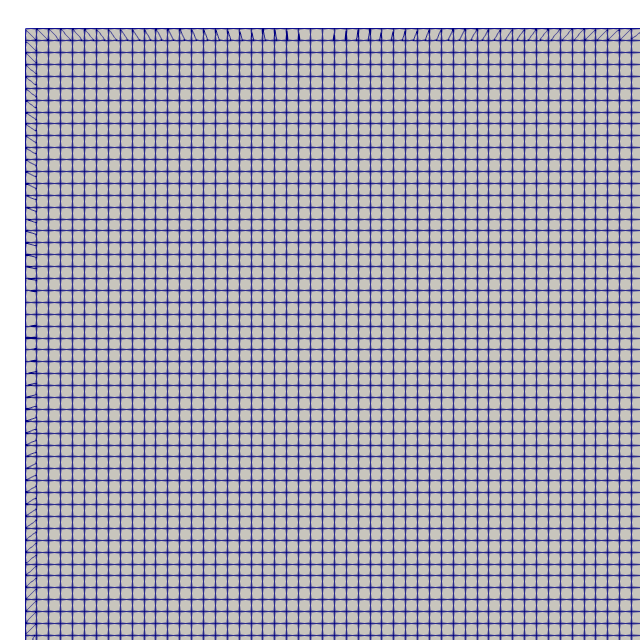
\includegraphics[width=.35\linewidth]{mesh_cavity.png}	
	\caption{Zoom of the computational mesh for the cavity.}
	\label{3.2fig}
\end{figure} 
The mesh is structured and consists of 1971212 nodes.

\subsection{Hypotheses And Assumptions}

\setlength{\parindent}{0.5cm} To carry out the current problem, a series of assumptions are taken into account in order to simplify the solving of the fluid equations involved.

\textbf{Laminar regime:} The Reynolds number, computed from the maximum velocity is not high enough to consider turbulent effects. 

\textbf{Convective heat transfer:} To determine whether the heat transfer is assumed to be convective, the Prandtl number and the Rayleigh number should be assessed.

\noindent The Prandtl number, as the relation between the viscosity and the thermal conductivity of a fluid or, in other words, the correlation between momentum transport and thermal transport capacity is calculated as:
\begin{equation}
	\operatorname{Pr}=\frac{v}{\alpha}=\frac{\mu}{\rho \alpha}=\frac{\mu c_{p}}{\lambda}=\frac{\text { momentum transport }}{\text { heat transport }}
	\label{3.3}
\end{equation}
where $\mu$ is the dynamic viscosity, $c_{p}$ is the specific heat and $\lambda$ is the thermal conductivity.

\noindent Thus, a small Prandtl number are owned by free-flowing flows with high thermal conductivitiy.

\noindent On the other hand, the Rayleigh number is referred to the time scale relation between the diffusive and the convective thermal transports. It is thus used to determine wheter the buoyancy-driven natural convection plays an important role in the heat transfer. The dimensionless number is assessed in this context by this form:
\begin{equation}
	\mathrm{Ra}_{x}=\frac{g \cdot \beta}{\nu \cdot \alpha} \cdot\left(T_{s}-T_{\mathrm{inf}}\right) \cdot x^{3}
	\label{3.4}
\end{equation}
Being \textit{g}, the gravity, \textit{$\beta$}, the coefficient of thermal expansion, \textit{$\nu$}, the kinematic viscosity, \textit{$\alpha$}, the thermal diffusivity, and \textit{$T_{s}$} and \textit{$T_{\mathrm{inf}}$}, the temperature on the wall surface and the temperature of the fluid far from the wall accordingly.

\noindent In the current case-scenario, a Prandtl close to 7 and a Rayleigh of 2517629 determine a convective heat transfer. The values used to estimate the Rayleigh number calculation are: $\beta = 6.734e-5 K^{-1}$, $\nu = 1.003e-6 m^{2}.s^{-1}$, $\alpha = 1.435e-7 m^{2}.s^{-1}$, $T_{s} = 283 K$, $T_{inf} = 273 K$ and $x = 0.038 m$. The values used for the laminar Prandtl number calculation are: $\mu = 0.001003 Kg.m^{-1}.s^{-1}$, $\lambda = 0.6 W.m^{-1}.K^{-1}$ and $C_{p}=4182 J.Kg.K^{-1}$.

\textbf{Newtonian fluid:} The viscosity of the fluid is assumed to be constant.

\textbf{Thermophysical properties:} specific heat, \textit{$C_p$}, the thermal expansion coefficient, \textit{$\beta$}, thermal conductivity, \textit{$\kappa$}, kinematic viscosity, \textit{$\nu$} are assumed to be non-dependent of temperature. However, the density will be dependent of temperature so as it plays an important role in the buoyancy effects through the later explained in this section.

\noindent The conservative equations used to describe the motion of the fluid along time and space are described next.

\subsection{Governing Equations}

\setlength{\parindent}{0.5cm} In this section, the governing equations for the used solver are described first.

The conservation of mass states that the mass flowing into the volume of control (CV) must be equal to the mass flowing out of such volume. 
\begin{equation}
	\frac{\partial v}{\partial y}+\frac{\partial w}{\partial z}=0
	\label{3.5}
\end{equation}

\subsubsection{Momentum Equation}

\setlength{\parindent}{0.5cm} Throughout the CV the momentum of the fluid flow is preserved and here below it is expressed for the y-direction and z-direction.
\begin{equation}
	\begin{aligned}
		\frac{\partial(\rho v)}{\partial t}+\operatorname{div}(\rho \mathbf{u} v)=\operatorname{div}(\mu \operatorname{grad} v)-\frac{\partial P}{\partial y}
	\end{aligned}
	\label{3.6}
\end{equation}
\begin{equation}
	\begin{aligned}
		\frac{\partial(\rho w)}{\partial t}+\operatorname{div}(\rho \mathbf{u} w)=\operatorname{div}(\mu \operatorname{grad} w)-\frac{\partial P}{\partial z}+S_{b}
	\end{aligned}
	\label{3.7}
\end{equation}
where in the case of the \textit{Boussinesq approximation} where the density variation is linear:
\begin{equation}
	S_{b} = g\cdot\rho_{r}[1-\beta(T-T_{r})]
	\label{3.8}
\end{equation}
in the case of the implemented polynomial density which accounts for the inversion point as in \cite{bourdillon_2016}:
\begin{equation}
	S_{b} = g\cdot[\rho_{r}-\rho(T)]
	\label{3.9}
\end{equation}
where the polynomial expression from $\rho$ is:
\begin{equation}
	\begin{aligned}
		\rho(T) &=999.840281167108+0.0673268037314653 \times T \\
		&-0.00894484552601798 \times T^{2} \\
		&+8.78462866500416 .10^{-5} \times T^{3} 
		-6.62139792627547 .10^{-7} \times T^{4}
	\end{aligned}
	\label{3.10}
\end{equation}
As it will be pointed out later, the native solver uses the Boussinesq approximation to account for the buoyancy effects. However, this linear assumption is only valid as the density variations meet:
\begin{equation}
	\frac{\Delta \rho}{\rho_{r}}<<1
	\label{3.11}
\end{equation}
Therefore, to account for the inversion points present during the freezing process, a density variation like the described in Eq. \ref{3.10} is implemented in the solver.

\subsubsection{Temperature Equation}
\setlength{\parindent}{0.5cm} The temperature equation representing the convection phenomena yields as:
\begin{equation}
	\begin{aligned}
	\frac{\partial T}{\partial t}+ \frac{\partial (u_{j} T)}{\partial x_{j}}=\frac{\partial}{\partial x_{j}}\left(\gamma \frac{\partial T}{\partial x_{j}}\right)
	\end{aligned}
	\label{3.12}
\end{equation}

where the thermal diffusivity, $\gamma$, is defined as:
\begin{equation}
	\gamma=\frac{\lambda}{\rho_{r} c_{p}}
	\label{3.13}
\end{equation}

All these equations are regarded by the solver \textit{buoyantBoussinesqPimpleFoam}.

\subsection{Solver descripton. Control Loop}

\setlength{\parindent}{0.5cm} The \textit{buoyantBoussinesqPimpleFoam} is a solver used to solve non-steady buoyancy driven fluids by using the Boussinesq approximation as a coupling between density and temperature fields. It considers the fluid as incompressible and uses the PIMPLE algorithm for the pressure-velocity coupling. The flowchart of the integration procedure for the presented solvers \textit{buoyantBoussinesqPimpleFoam} and \textit{icoReactingMultiphaseinterFoam} is presented below:

\tikzstyle{decision} = [diamond, draw, fill=blue!20,
text width=4.5em, text badly centered, node distance=2.5cm, inner sep=0pt]
\tikzstyle{block} = [rectangle, draw, fill=blue!20,
text width=5em, text centered, rounded corners, minimum height=4em]
\tikzstyle{line} = [draw, very thick, color=black!50, -latex']
\tikzstyle{cloud} = [draw, ellipse,fill=red!20, node distance=2.5cm,
minimum height=2em]

\begin{figure}[h!]
	\centering
	\begin{tikzpicture}[scale=1.5, node distance = 2cm, auto]
	% Place nodes
	\node [block] (init) {Velocity predictor};
	\node [block, below of=init] (identify) {Temperature Equation};
	\node [block, below of=identify] (evaluate) {Pressure Equation};
	\node [block, below of=evaluate] (update) {Velocity Corrector};
	\node [block, left of=evaluate, node distance=3cm] (update1) {PIMPLE LOOP};
	\node [block, right of=evaluate, node distance=3cm] (update2) {PISO LOOP};
	\node [decision, below of=update] (decide) {Residuals satisfied?};
	\node [block, below of=decide, node distance=2.5cm] (stop) {stop};
	% Draw edges
	\path [line] (init) -- (identify);
	\path [line] (identify) -- (evaluate);
	\path [line] (evaluate) -- (update);
	\path [line] (update) -- (decide);
	\path [line] (decide) -| node [near start, color=black] {no} (update1);
	\path [line] (update1) |- (init);
	\path [line] (update) -| node [near start, color=black] {} (update2);
	\path [line] (update2) -- (evaluate);	
	\path [line] (decide) -- node [, color=black] {yes}(stop);
	
	\end{tikzpicture}
	\label{3.3fig}
	\caption{Flowchart of integration procedure. \textit{buoyantBoussinesqPimpleFoam}}
\end{figure}

\subsection{Code implementations}

\setlength{\parindent}{0.5cm} As described in the \textit{Governing equations} section, the need for a polynomial density expression and a variation of the momentum source terms devoted to reflect the buoyancy effects is derived.

\noindent To do so, a new equation of state is implemented within the OpenFoam framework. Now and, in order to take into account this bouyancy forces, the pressure equation is studied. This is beacause in the context of a pressure-velocity corrector scheme, and in the case of ensuring stability and simplifying the boundary conditions definition, the modified pressure, \textit{$p_{rgh}$}, within the pressure equation implementation, is the term that accounts for the gravity terms.

\noindent Here, it is presented a general form of a momentum equation with the continuity equation corresponding to a incompressible flow.  
\begin{equation}
	\left\{\begin{array}{l}
	\frac{\partial (\rho \textbf{v})}{\partial t}+\nabla \cdot(\rho \textbf{v} \otimes \textbf{v})=-\nabla p+ \nabla \cdot(\mu (\nabla \textbf{v}+\nabla \textbf{v}^{T})) \\
	\nabla \cdot \textbf{v}=0
	\end{array}\right.
	\label{3.14}
\end{equation}
From this general equation, it will be given the term $H(\textbf{u})$, as later on will be needed for the pressure equation calculation.

\noindent Therefore, this term comes from considering the linearization of the advective term under the assumption of small Courant numbers (Co < 1). Leading the term $\textbf{v}^{0}\cong\textbf{v}$. 
\begin{equation}
	\begin{aligned}
	\int_{\Omega} \nabla \cdot\left(\textbf{v} \otimes \textbf{v}^{0}\right) d \Omega & \cong \sum_{f} \textbf{v}_{f} \textbf{v}_{f}^{0} \cdot \textbf{S}_{f} \\
	&=\sum_{f} F^{0} \textbf{v}_{f} \\
	&=a_{P} \textbf{v}+\sum_{f} a_{N} \textbf{v}_{N}
	\end{aligned}
	\label{3.15}
\end{equation}

\begin{equation}
	a_{P} \textbf{v}_{P}=\textbf{H}(\textbf{v})-\nabla p
	\label{3.16}
\end{equation}
\begin{equation}
	\textbf{H}(\textbf{v})=\underbrace{-\sum_{f} a_{N} \textbf{v}_{N}}_{\text {Diagonal term }}+\underbrace{\frac{\textbf{v}^{0}}{\Delta t}}_{\text {Off-diagonal term }}
	\label{3.17}
\end{equation}
where $\textbf{v}^{0}$ is the velocity at previous time-step and $F^{0}$ is the face flux at the previous time-step.

\noindent In addition, by discretizing the continuity equation, it is possible to get the final form of the pressure equation.

\noindent So as to give stability to the solution and to simplify the boundary conditions definition as described in Berberovic et al. \cite{berberovic_van_hinsberg_jakirlic_roisman_tropea_2009}, a modified pressure is defined as,
\begin{equation}
	p_{r g h}=p-\rho_{r} \textbf{g} \cdot \textbf{x} + \rho(T) \textbf{g} \cdot \textbf{x}
	\label{3.18}
\end{equation}
being, the pressure gradient the next expression,
\begin{equation}
	-\nabla p+\rho_{r} \textbf{g}=-\nabla p_{r g h}-\textbf{g} \cdot \textbf{x} \nabla \rho_{r} + \textbf{g} \cdot \textbf{x} \nabla \rho(T) + \rho(T) \textbf{g}
	\label{3.19}
\end{equation}
and rearranging terms, 
\begin{equation}
	-\nabla p+\rho_{r} \textbf{g} + \textbf{g} \cdot \textbf{x} \nabla \rho_{r} - \textbf{g} \cdot \textbf{x} \nabla \rho(T) - \rho(T) \textbf{g}=-\nabla p_{r g h}
	\label{3.20}
\end{equation}
If one tries to describe the discretized pressure equation in \textit{buoyantBoussinesqPimpleFoam}, there is a first term called \textbf{phig}, which is,
\begin{equation}
	\Phi_{f}^{\nu+1}=\Phi_{u}^{\nu+1} - \left[(\textbf{g} \cdot \textbf{x})_{f}\left(\nabla \rho_{r}{ }^{n+1}\right)_{f}+(\textbf{g} \cdot \textbf{x})_{f}\left(\nabla \rho(T){ }^{n+1}\right)_{f}\right]\frac{\left|\textbf{S}_{f}\right|}{\left(a_{P}\right)_{f}}
	\label{3.21}
\end{equation}
This term is edited in the code so as it handles the new expression for the buoyancy effects as regarded by Bourdillon, \cite{bourdillon_2016}.

A face flux calculated by the term \textbf{H}(\textbf{v}), appearing in equation \ref{3.17}
\begin{equation}
	\Phi_{u}^{\nu+1}=\Phi_{f}^{\nu+1} + \left(\frac{H\left(\textbf{v}^{\nu}\right)}{a_{P}}\right)_{f} \cdot \textbf{S}_{f}+\left(\frac{1}{a_{P}}\right)_{f}\operatorname{ddt} \operatorname{PhiCorr}\left(\textbf{v}^{\nu}, \Phi^{\nu}\right)
	\label{3.22}
\end{equation}
where $\operatorname{ddt} \operatorname{PhiCorr}$ is a flux adjustment due to the time-step. This is resolved by applying a \textit{Rhie-Chow interpolation} \cite{rhie_chow_1983}, the next term in the pressure equation, \textbf{phiHbyA}, reads as,
\begin{equation}
	\Phi_{f}^{\nu+1}=\Phi_{f}^{\nu+1}-\left[\left(\frac{1}{a_{P}}\right)_{f}\left(\nabla p_{r g h}\right)_{f}\right] \cdot \textbf{S}_{f}
	\label{3.23}
\end{equation}
The \textbf{$p_{rgh}$} term is thus assembled as,
\begin{equation}
	\sum_{f}\left[\left(\frac{1}{a_{P}}\right)_{f}\left(\nabla p_{r g h}^{\nu+1}\right)_{f}\right] \cdot \textbf{S}_{f}=\sum_{f} \Phi^{\nu+1}
	\label{3.24}
\end{equation}
The flux, \textit{$\phi$}, is adjusted by the \textbf{$p_{rgh}$} term yielding the following expression,
\begin{equation}
	\Phi_{f}^{\nu+1}=\Phi_{f}^{\nu+1}-\left[\left(\frac{1}{a_{P}}\right)_{f}\left(\nabla p_{r g h}\right)_{f}\right] \cdot \textbf{S}_{f}
	\label{3.25}
\end{equation}
\begin{equation}
	\begin{aligned}
		\Phi_{f}^{\nu+1}=&\Phi_{f}^{\nu+1}+\biggl[\left(\frac{1}{a_{P}}\right)_{f}\biggl[(-\nabla p)_{f}+ (\textbf{g} \cdot \textbf{x})_{f}\left(\nabla \rho_{r}{ }^{n+1}\right)_{f}-(\textbf{g} \cdot \textbf{x})_{f}\left(\nabla \rho(T){ }^{n+1}\right)_{f}\\
		&+ (\rho_{r}{ }^{n+1} \textbf{g})_{f}-(\rho(T){ }^{n+1} \textbf{g})_{f} \biggr]\biggr] \cdot \textbf{S}_{f}
	\end{aligned}
	\label{3.26}
\end{equation}
Finally, the velocity calculated at the center of the volume reads as,
\begin{equation}
	\textbf{v}^{\nu+1}=\textbf{v}^{\nu+1} +\frac{1}{a_{P}}\mathcal{R}\left[\left(\Phi^{\nu+1} f-\Phi_{u}^{\nu+1} f\right)\left(a_{P}\right)_{f}\right]
	\label{3.27}
\end{equation}
where $\mathcal{R}$ is an operator used to recover cell-centered fields from fields given as fluxes at faces.
Then, the static pressure, \textit{p}, is reconstructed from \textit{$p_{rgh}$}, leading the expression,

\begin{equation}
	p = p_{r g h} + (\rho_{r}-\rho(T))\textbf{g}\cdot \textbf{x}
	\label{3.28}
\end{equation}
 
\subsection{Case Setup}

\setlength{\parindent}{0.5cm} Once the implementation is done, a first case is studied with the existing solver, \textit{buoyantBoussinesqPimpleFoam}. Later, the same case is settled with the new implementations.
The boundary conditions, thermophysical properties and some other solver parameters are described along the following subsections.
\newline
As commented before, all studies are calculated on a computational domain of \textit{38mm x 38mm}. 
\begin{figure}[h]
	\label{3.4fig}	\centering	
	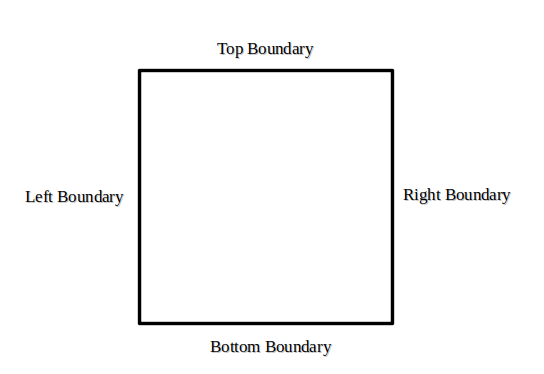
\includegraphics[width=0.6\textwidth]{domain.png}
	\caption{Setting of cavity computational domain.}
\end{figure} 

\subsubsection*{Boundary conditions}
\setlength{\parindent}{0.5cm} Five boundaries are defined in the current case:
\newline
\textbf{Left:} is considered a wall with a fixed value of temperature. This is the hot wall. No velocity is prescribed.
\newline
\textbf{Right:} considered to be the cold wall with a fixed temperature. No velocity is prescribed.
\newline
\textbf{Top:} this is considered the top wall and it is adiabatic, thus, no heat transfer is assumed and zero gradient is applied. No velocity is applied.
\newline 
\textbf{Bottom:} This shares similar conditions as the top wall.
\newline
\textbf{frontAndBack:} this uses a symmetry plane condition in the z direction since the problem is considered to be 2-dimensional. For such boundary type, no more conditions need to be prescribed.
\begin{table}[h!]
	\begin{tabular}{@{}lllll@{}}
		\toprule[1pt]
		\textbf{Boundary} & \textbf{Conditions}  \\ \midrule[2pt]
		Left & $T_{l}=283, v_{l} = 0   $  \\
		Right & $T_{r}=273, v_{r} = 0 $ \\
		Top & $\frac{\partial T_{u}}{\partial n} = 0, v_{u} = 0$  \\
		Bottom & $\frac{\partial T_{b}}{\partial n} = 0, v_{b} = 0$  \\ \bottomrule[1pt]		
	\end{tabular}
	\centering
	\caption{Boundary conditions for natural convection case.}	
	\label{3.2tab}
\end{table}
\newline

\subsubsection*{Thermophysical properties}
The thermophysical properties for the natural convection calculation are described in \ref{3.3tab}. 
\begin{table}[h!]
	\begin{tabular}{@{}lllll@{}}
		\toprule[1pt]
		\textbf{Water properties} & \textbf{Symbol} & \textbf{Values} & \textbf{Units} &  \\ \midrule[2pt]
		Density & $\rho_r$ & 999.8 & $kg.m^{-3}$ \\
		Dynamic viscosity & $\mu$ & 0.001003 & $kg.m^{-1}.s^{-1}$ \\
		Thermal conductivity & $\lambda$ & 0.6 & $W.m^{-1}.K^{-1}$ \\
		Heat capacity & $C_p$ & 4182 & $J.kg.K^{-1}$ \\		 
		Gravitational acceleration & $g$ &  9.81  & $m.s^{-2}$ \\
		Thermal diffusivity & $\gamma$ &  1.435e-7  & $m^{2}.s^{-1}$ \\		
		Thermal expansion coefficient & $\beta$ &  6.734e-5  & $K^{-1}$ \\	
		Laminar Prandtl number & $P_r$ &  6.99  & - \\
		Reference temperature & $T_r$ &  6.734e-5  & $K$ \\ \bottomrule[1pt]		
	\end{tabular}
	\centering
	\caption{Water properties for natural convection.}	
	\label{3.3tab}
\end{table}
\newline
Here below are presented the discretization schemes used for the terms appearing on the equations involved in the calculation. For more information on the used ones, refer to \cite{openfoamuserguide:cfddirect}.
\begin{table}[h!]
	\begin{adjustbox}{width=1\textwidth}
		\small	
		\begin{tabular}{@{}lllll@{}}
			\toprule[1pt]
			\textbf{Modeling Term} & \textbf{Keyword} & \textbf{Scheme} & \textbf{Remarks} &  \\ \midrule[2pt]
			Time derivatives & ddtSchemes    &  Euler  & First order, bounded, implicit \\
			Divergence term    & divSchemes   &    & Second order, unbounded \\
			Gradient term    & gradSchemes    &  Gauss linear  & Second order, unbounded \\
			Laplacian term   &  laplacianSchemes    &  Gauss linear orthogonal  & Second order \\		 
			Grad. normal to cell face & snGradSchemes    &  orthogonal  &  Second order\\ 
			Point to point interpolation&    			   interpolationSchemes    & linear   & Central differencing \\ \bottomrule[1pt]		
		\end{tabular}
	\end{adjustbox}
	\centering
	\caption{Discretization schemes.}	
	\label{3.4tab}
\end{table}
\clearpage
The equation solvers are shown in \ref{3.5tab}. 
\begin{table}[h!]
	\begin{tabular}{@{}lllll@{}}
		\toprule[1pt]
		\textbf{Equation} & \textbf{Linear Solver} & \textbf{Smoother/Preconditioner} & \textbf{Tolerance} &  \\ \midrule[2pt]
		Pressure correction equation & PCG & DIC & 1e-8 \\
		Momentum equation & PBiCGStab & DILU  & 1e-6 \\
		Temperature equation & PBiCGStab & DILU  & 1e-6 \\\bottomrule[1pt]		
	\end{tabular}
	\centering
	\caption{Solvers for the discretised equations.}	
	\label{3.5tab}
\end{table}
\newline
Table \ref{3.6tab} presents the parameters used for the inner and outter loops performed within the calculation.
\begin{table}[h!]
	\begin{tabular}{@{}lllll@{}}
		\toprule[1pt]
		\textbf{Parameter} & \textbf{Value} \\ \midrule[2pt]
%		nAlphaCorr & PCG & DIC &  \\
%		nAlphaSubCycles & smoothSolver & symGaussSeidel  &  \\
%		cAlpha & smoothSolver & symGaussSeidel  &  \\
		momentumPredictor &  no    &    &  \\		 
		nOuterCorrectors &  1   &    &  \\ 
		nNonOrthogonalCorrectors &  0   &    &  \\ 		
		nCorrectors & 2	&    &  \\ \bottomrule[1pt]		
	\end{tabular}
	\centering
	\caption{Parameters for the discretised equations.}	
	\label{3.6tab}
\end{table}

\clearpage
\subsection{Validation of Results and Conclusions}
For comparison purposes and so as to know the state of the art in the natural convection phenomena, a first analysis is performed using the convection solver provided by OpenFOAM. This solver is BuoyantBoussinesqPimpleFoam and it covers both laminar and turbulent unsteady heat transfer for single phase fluids using the Boussinesq approximation. Afterwards, the case is calculated with the new implementations described.
\begin{figure}[h!]
	\centering
	\begin{subfigure}{\linewidth}
	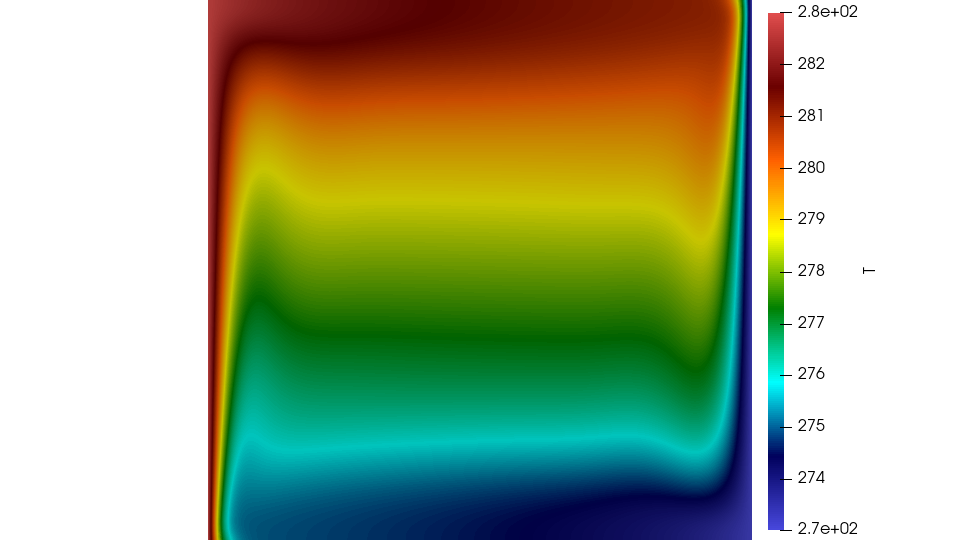
\includegraphics[width=.55\linewidth]{BBPF_T_1500s.png}\hfill
	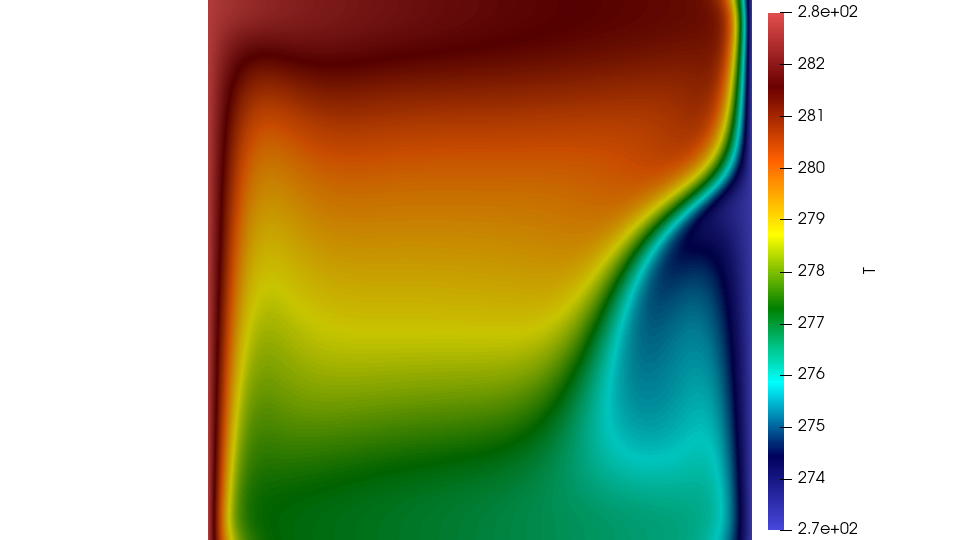
\includegraphics[width=.55\linewidth]{CF_T_1500s_comp.png}	
	\caption{Temperature magnitude comparison at t = 1500s. Left: BBPF. Right: mBBPF.}
	\label{3.5figa}
	\end{subfigure}\par\medskip
	\begin{subfigure}{\linewidth}
	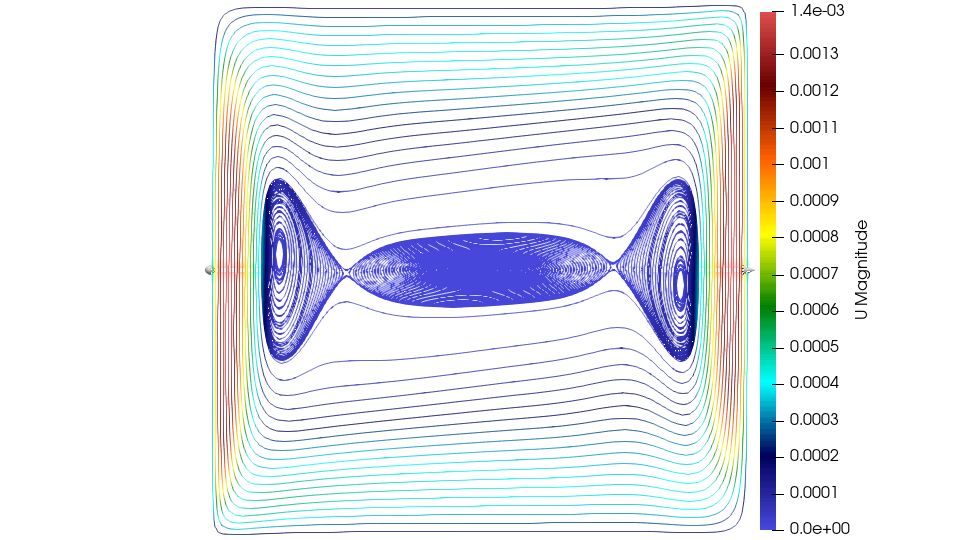
\includegraphics[width=.55\linewidth]{BBPF_U_1500s.png}\hfill
	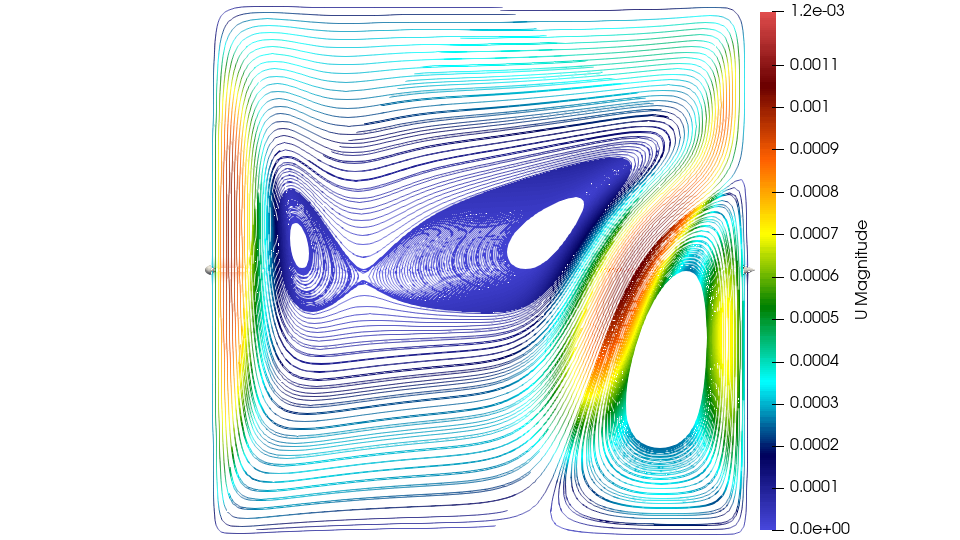
\includegraphics[width=.55\linewidth]{CF_U_1500s_comp.png}	
	\caption{Velocity magnitude comparison at t = 1500s. Left: BBPF. Right: mBBPF}
	\label{3.5figb}
	\end{subfigure}\par\medskip
	\caption{Comparison between BBPF* and mBBPF**}
	\label{3.5fig}
\end{figure}
\newline 
BBPF*: BuoyantBoussinesqPimpleFoam solver.
mBBPF**: myBuoyantBoussinesqPimpleFoam, natural convection modified solver.

\noindent The gravity terms of the temperature and velocity magnitude distributions shown in Fig. \ref{3.5fig} (left) are as expressed in Equation \ref{3.8}, $(S_{b} = g\cdot\rho_{r}[1-\beta(T-T_{r})])$. In addition, the equation of state used to describe the behavior of the liquid density variation is linear. On the other hand, the proposed gravity terms proposed by \cite{bourdillon_2016} and described in Equation \ref{3.9}, $(S_{b} = g\cdot[\rho_{r}-\rho(T)])$, besides of the polynomial density variation have depicted a non-linear pattern for the temperature and velocity magnitude distibutions. It is seen that small changes in the density, $0.171925 kg.m^-3$ in this case, Fig. \ref{rhodifffig}, may induce different patterns within the flow. 
\clearpage
\begin{figure}[h!]
	\centering
	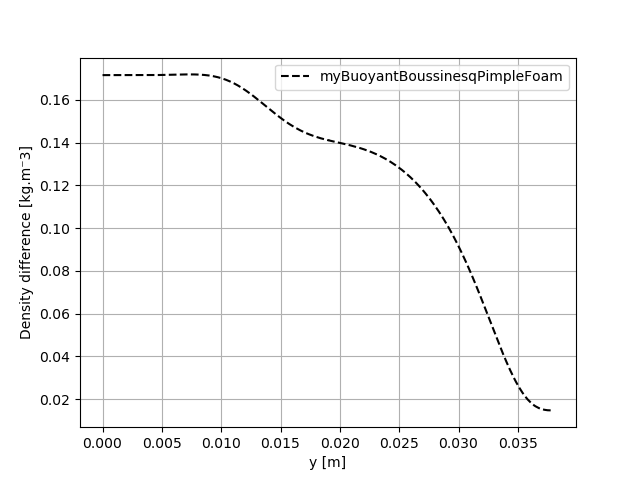
\includegraphics[width=.55\linewidth]{rhodiff_CF.png}\hfill
	\caption{Density differences between linear and polynomial expressions.}
	\label{rhodifffig}
\end{figure} 

\noindent The fact of achieving the description of the inversion point in the temperature distribution due to the density variation of the density will influence the growth of the ice layer in the phase change simulations.

\noindent Therefore, in order to compare consistently the obtained results with those of the literature, the following dimensionless values are pointed out:

\noindent Dimensionless values of temperature are described as:
\begin{equation}
	\tilde{T}=\frac{T-T_{\text {cold }}}{T_{\text {hot }}-T_{\text {cold }}}=\frac{T-273}{10}
	\label{3.29}
\end{equation}
Horizontal and vertical dimensionless positions along the x and y mid-planes:
\begin{equation}
	\tilde{x}=\frac{x}{\ell}=\frac{x}{38 \times 10^{-3}}
	\label{3.30}
\end{equation}
\begin{equation}
\tilde{y}=\frac{y}{\ell}=\frac{y}{38 \times 10^{-3}}
\label{3.34}
\end{equation}
Transversal and axial dimensionless velocities:
\begin{equation}
	\tilde{v}=\frac{v \ell}{\gamma}=\frac{v 38 \times 10^{-3}}{1.435 \times 10^{-7}}
	\label{3.31}
\end{equation}
\begin{equation}
	\tilde{u}=\frac{u \ell}{\gamma}=\frac{u 38 \times 10^{-3}}{1.435 \times 10^{-7}}
	\label{3.32}
\end{equation}

\clearpage
\noindent The presented dimensionless quantities obtained with the gravity related terms implemented in the convection solver are compared against the literature. Bourdillon et al. \cite{bourdillon_2016} used as a reference and guideline, worked out a solution using OpenFOAM and Kowalewski et al. \cite{kowalewski_rebow_1999} who in 1999 performed similar calculations using Fluent.

\noindent The results obtained with myBuoyantBoussinesqPimpleFoam, the natural convection modified solver, show acceptable agreement with the results found in the literature. The highest local differences are found in the V-velocity along the vertical direction, Fig. \ref{3.6ffig}. The relative error of the proposed numerical solution with respect to the one shown in Kowaleswki et al. remains below 16\%. Moreover, as it is observable, the temperature dimensionless, Fig. \ref{3.6bfig}, distribution and the U-velocity, Fig. \ref{3.6dfig}, plotted along the vertical mid-plane seem to be in short disaccordance with respect to the literature's solutions. This differences might be due to a small shift of the dimensionless magnitudes along that direction. However, in overall, the results nearly overlap the ones found in the bibliography.
\clearpage
\begin{figure}[h!]
	\begin{subfigure}{0.50\textwidth}
		\centering
		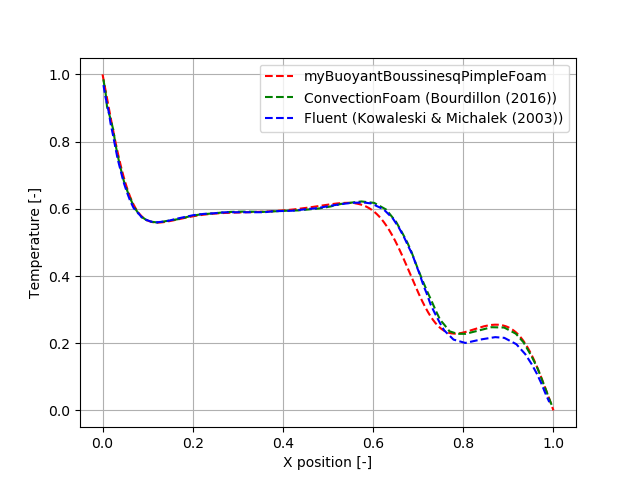
\includegraphics[width=\linewidth]{temperature_xpos_conv.png}\hfill
		\caption{Temperature along horizontal line.} \label{3.6afig}
	\end{subfigure}
	\hfill
	\begin{subfigure}{0.50\textwidth}
		\centering
		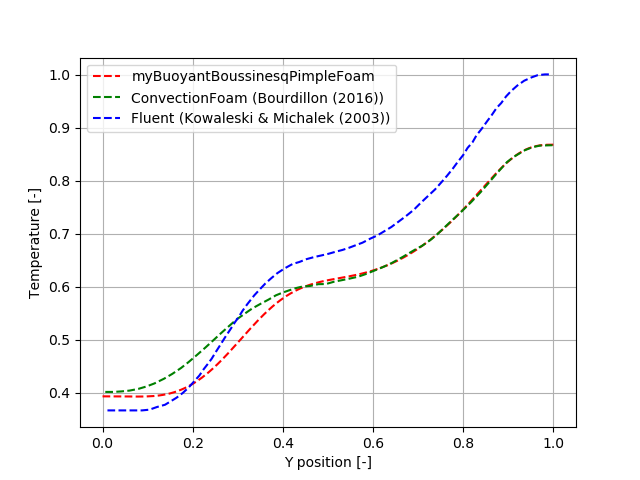
\includegraphics[width=\linewidth]{temperature_ypos_conv.png}	
		\caption{Temperature along vertical line.}\label{3.6bfig}
	\end{subfigure}
	\begin{subfigure}{0.50\textwidth}
		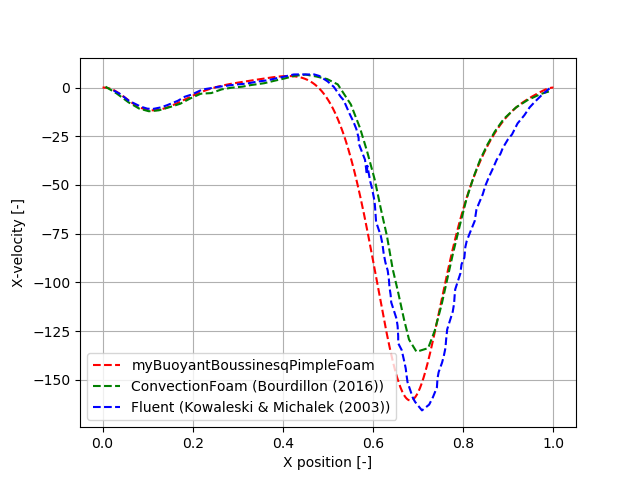
\includegraphics[width=\linewidth]{xvel_xpos_conv.png}\hfill
		\caption{U-velocity along horizontal line.}\label{3.6cfig}
	\end{subfigure}
	\begin{subfigure}{0.50\textwidth}
	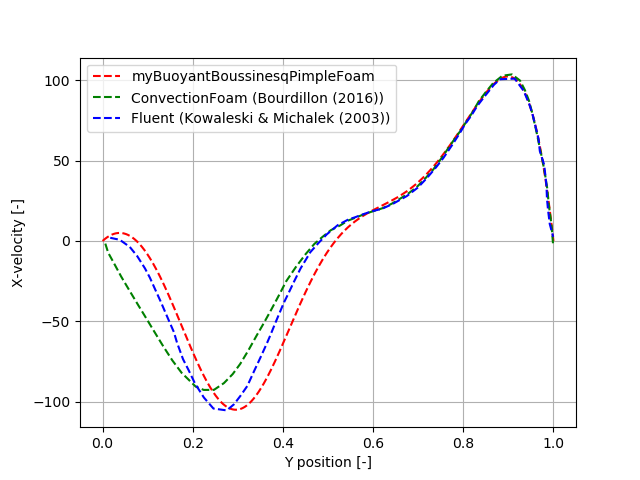
\includegraphics[width=\linewidth]{xvel_ypos_conv.png}	
	\caption{U-velocity along vertical line.}\label{3.6dfig}
	\end{subfigure}
	\begin{subfigure}{0.50\textwidth}
	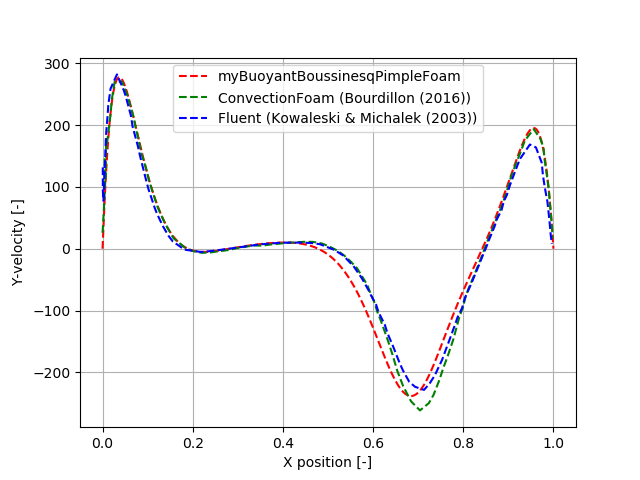
\includegraphics[width=\linewidth]{yvel_xpos_conv.png}\hfill	
	\caption{V-velocity along horizontal line.}\label{3.6efig}
	\end{subfigure}
	\begin{subfigure}{0.50\textwidth}
	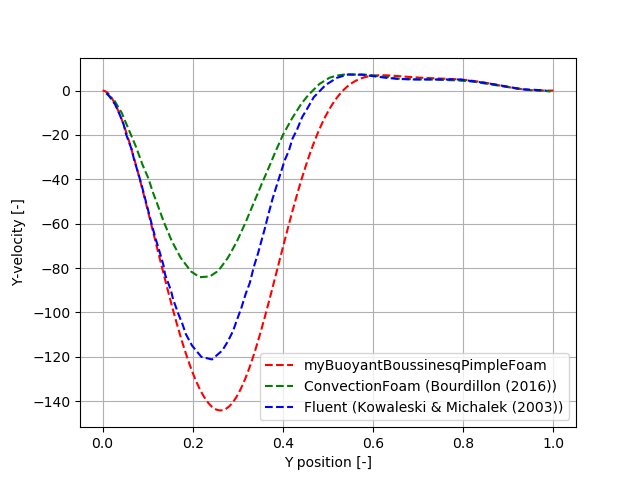
\includegraphics[width=\linewidth]{yvel_ypos_conv.png}	
	\caption{V-velocity along vertical line.}\label{3.6ffig}
	\end{subfigure}
	\caption{Adimensional magnitudes comparison.}
	\label{3.6fig}
\end{figure} 

In the table \ref{3.7tab}, there are shown the temperature, velocity magnitude and density distributions at different time steps. From these images, it can be understood the physical phenomena arising in the natural convection of the problem proposed. At time 100s, the left wall, initiallized at 283K, induces the propagation of the hottest flow through the volume of control and towards the right wall which is initially at 273K. Through time, it is observable how the coldest flow and thereby the less dense, is driven to the bottom region of the cavity while the denser one is redirected over the top. Another remarkable fact is that two flows are originated due to this density inversion point. One emerged near the left wall which moves clockwise and the other one arisen in the mid-bottom part of the right wall which moves on the opposite direction, thus, counter clockwise. This phenomena exhibits by the fact that the density variation is characterized by a polynomial function and it is of importance since this behavior has an impact in the ice layer formation.
\begin{table}[h!]
	\begin{tabular}{@{}lllll@{}}
		\toprule[1pt]
		\multicolumn{1}{c}{\textbf{t = 100s}} & \multicolumn{1}{c}{\textbf{t = 250s}} & \multicolumn{1}{c}{\textbf{t = 1500s}} \\ \midrule[2pt] 
		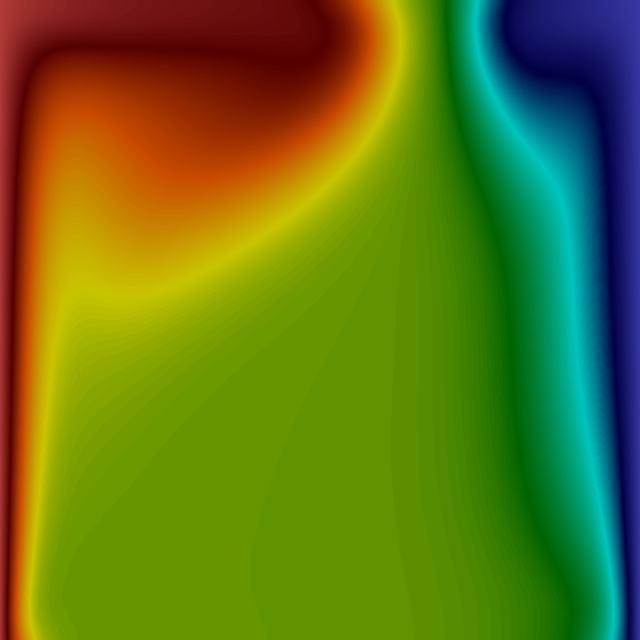
\includegraphics[width=.25\linewidth]{CF_T_100s.png} & 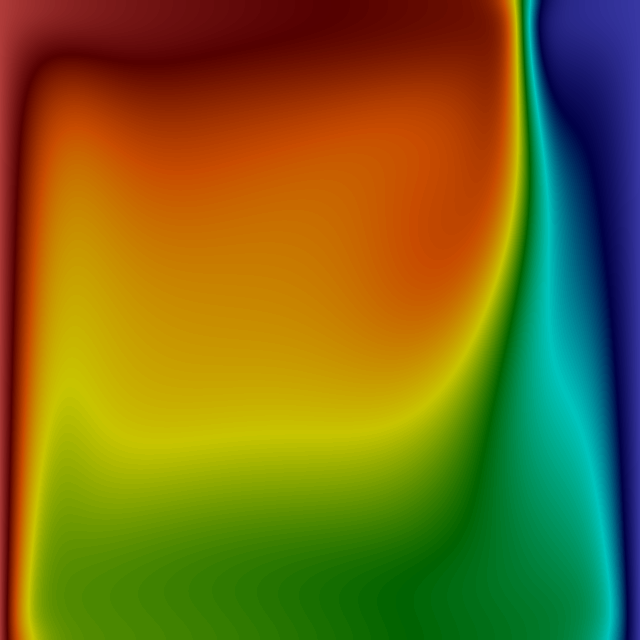
\includegraphics[width=.25\linewidth]{CF_T_250s.png} & 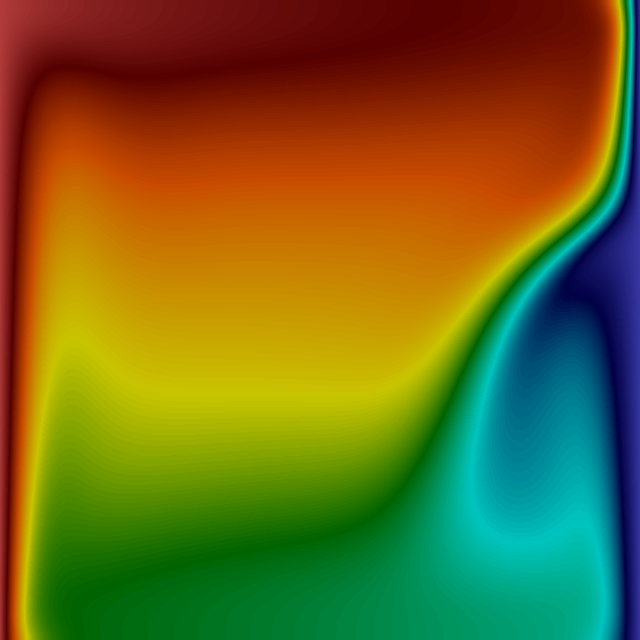
\includegraphics[width=.25\linewidth]{CF_T_1500s.png} & 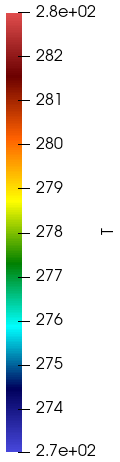
\includegraphics[width=.0658\linewidth]{t.png} \\
		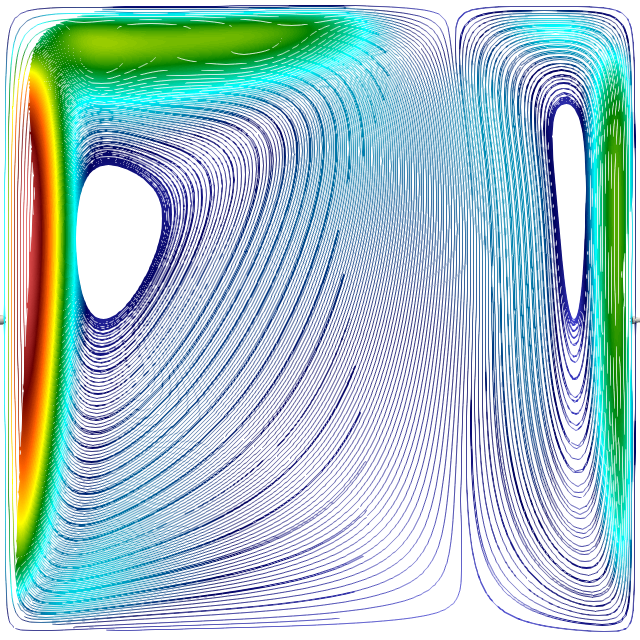
\includegraphics[width=.25\linewidth]{CF_U_100s.png} & 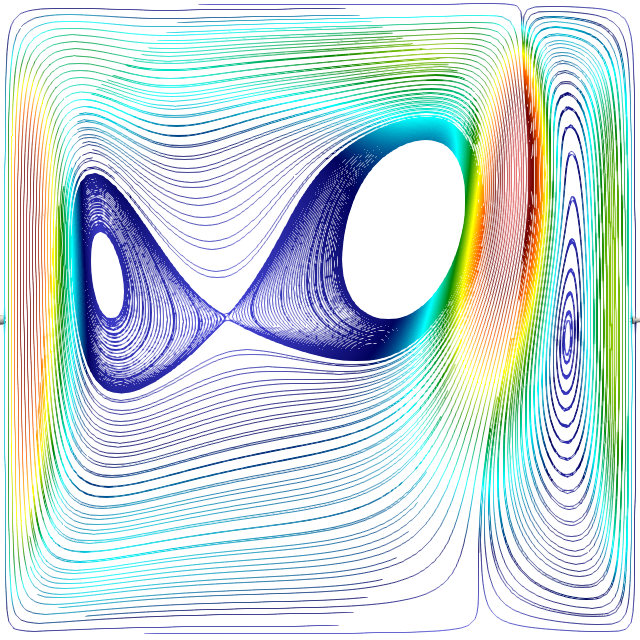
\includegraphics[width=.25\linewidth]{CF_U_250s.png} & 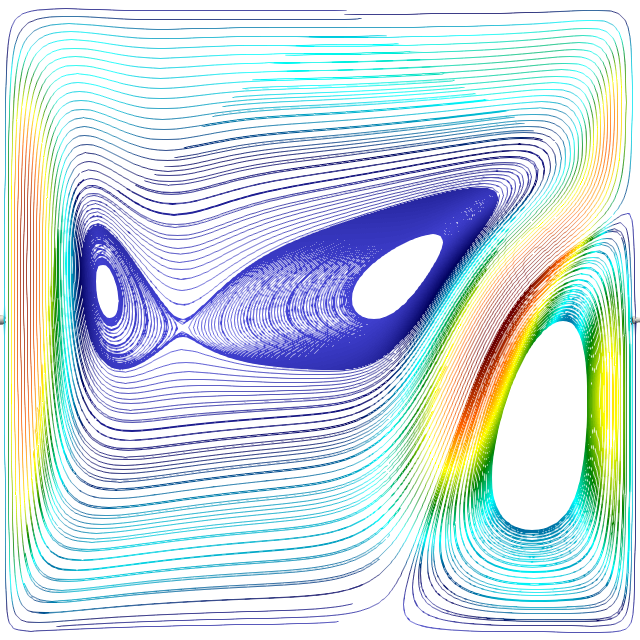
\includegraphics[width=.25\linewidth]{CF_U_1500s.png} & 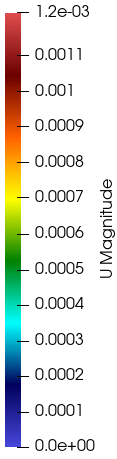
\includegraphics[width=.0658\linewidth]{u.png} \\
		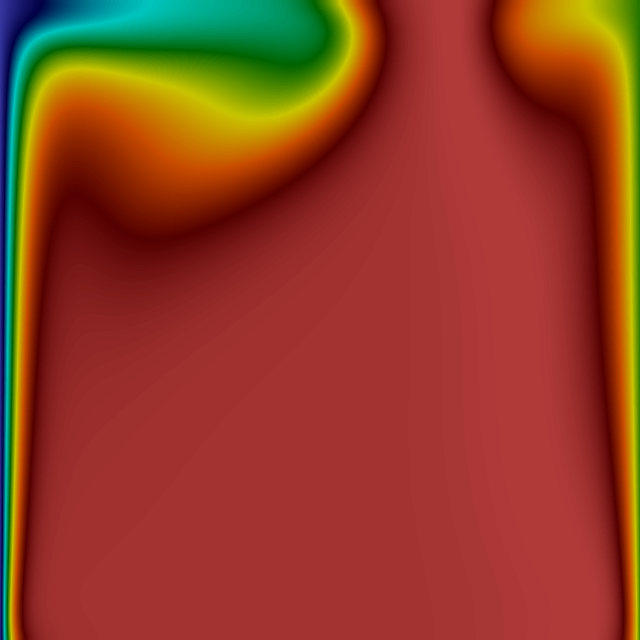
\includegraphics[width=.25\linewidth]{CF_rho_100s.png} & 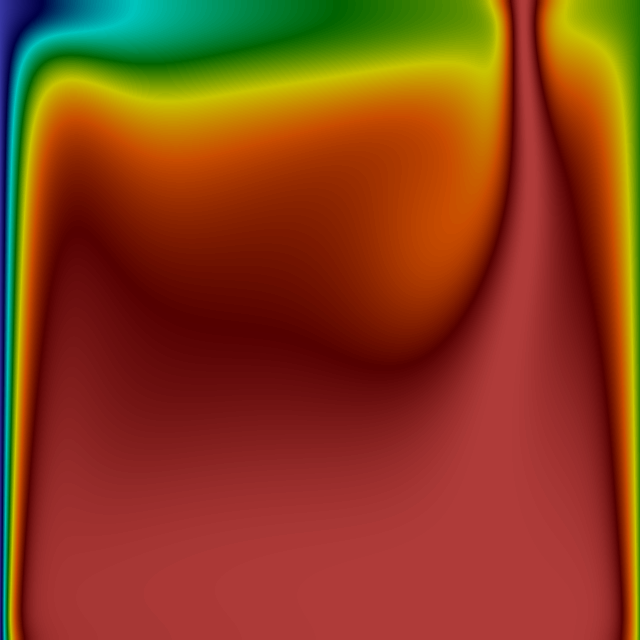
\includegraphics[width=.25\linewidth]{CF_rho_250s.png} & 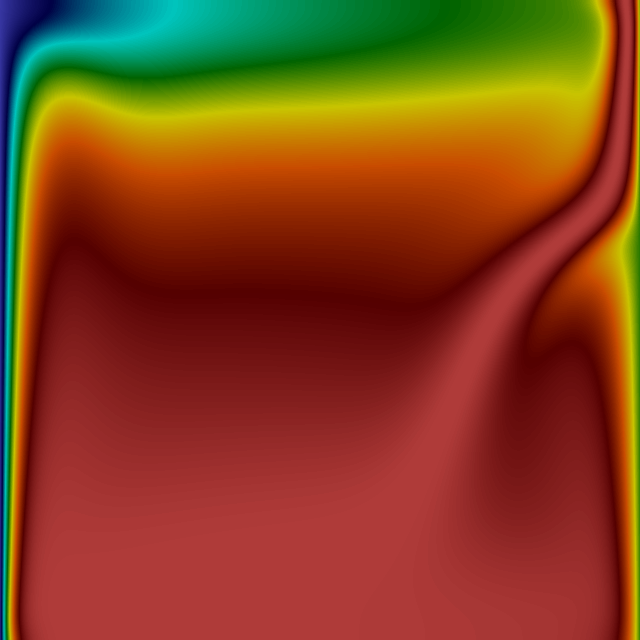
\includegraphics[width=.25\linewidth]{CF_rho_1500s.png} & 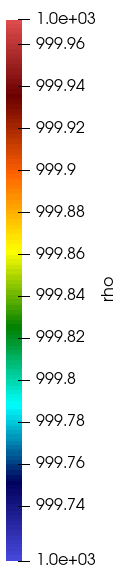
\includegraphics[width=.0558\linewidth]{rho.png} \\ \bottomrule[1pt]		
	\end{tabular}
	\centering
	\caption{Numerical results of natural convection modified solver between \textit{t = 100s} and \textit{1500s}.}	
	\label{3.7tab}
\end{table}
\newline
\noindent In the table shown below are compared the temperature, velocity magnitudes and density distributions for \textit{t = 750s} and \textit{1500s}. As it is observable, between these time steps, the magnitudes do not change substantially and, therefore, one could say that a quasy-steady state is obtained. The solution at \textit{1500s} is used as initial condition for the process of solidification. In the next chapter is commented the concept behind this assumption.
\begin{table}[h!]
	\begin{tabular}{@{}lllll@{}}
		\toprule[1pt]
		\multicolumn{1}{c}{\textbf{t = 750s}} & \multicolumn{1}{c}{\textbf{t = 1500s}} \\ \midrule[2pt] 
		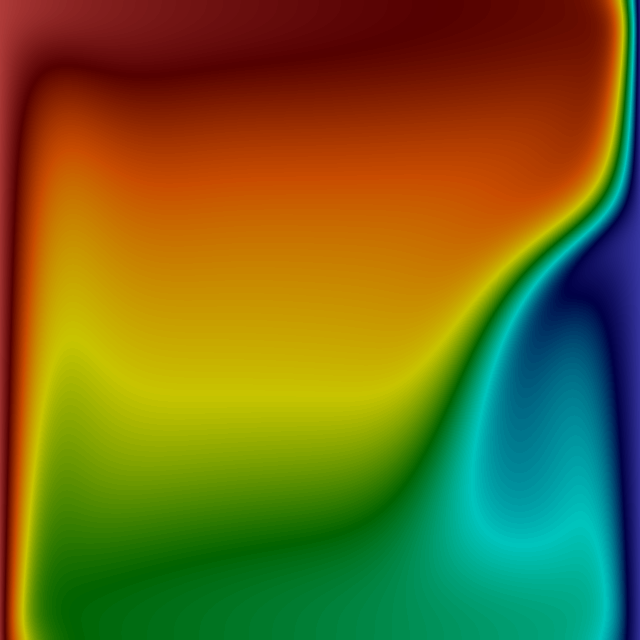
\includegraphics[width=.25\linewidth]{T_750s_CF.png} & 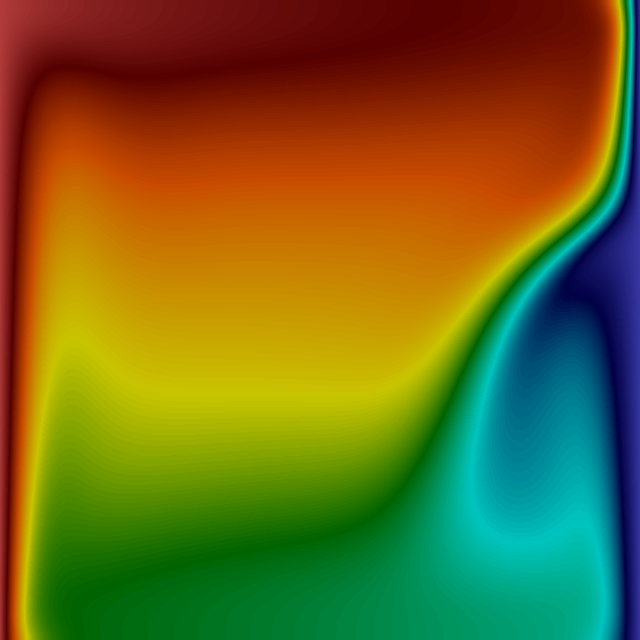
\includegraphics[width=.25\linewidth]{CF_T_1500s.png} & 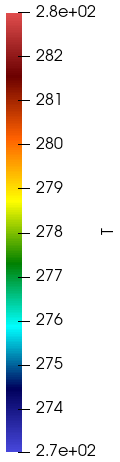
\includegraphics[width=.0658\linewidth]{t.png} \\
		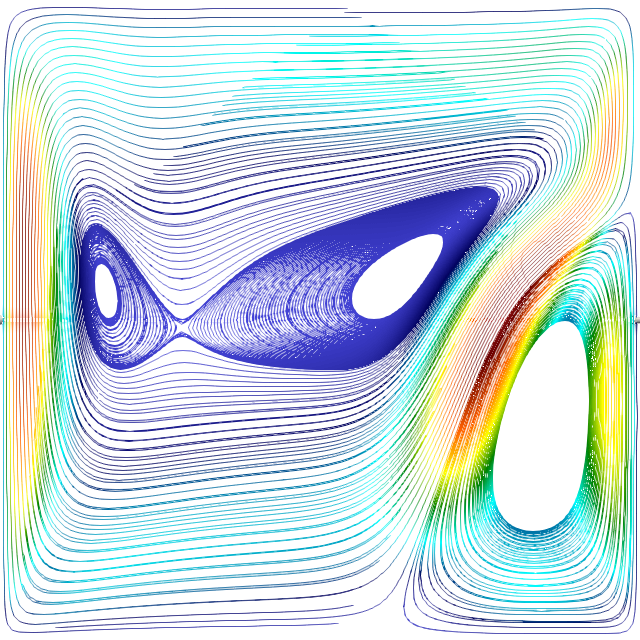
\includegraphics[width=.25\linewidth]{U_750s_CF.png} &  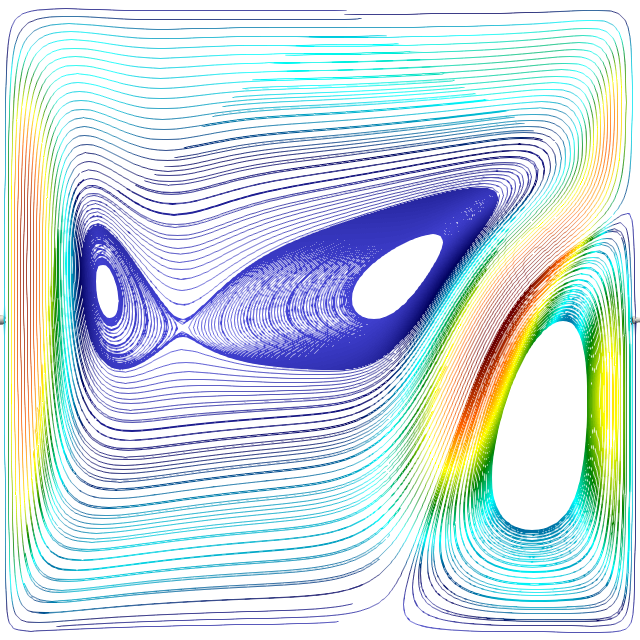
\includegraphics[width=.25\linewidth]{CF_U_1500s.png} & 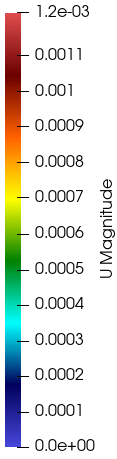
\includegraphics[width=.0658\linewidth]{u.png} \\
		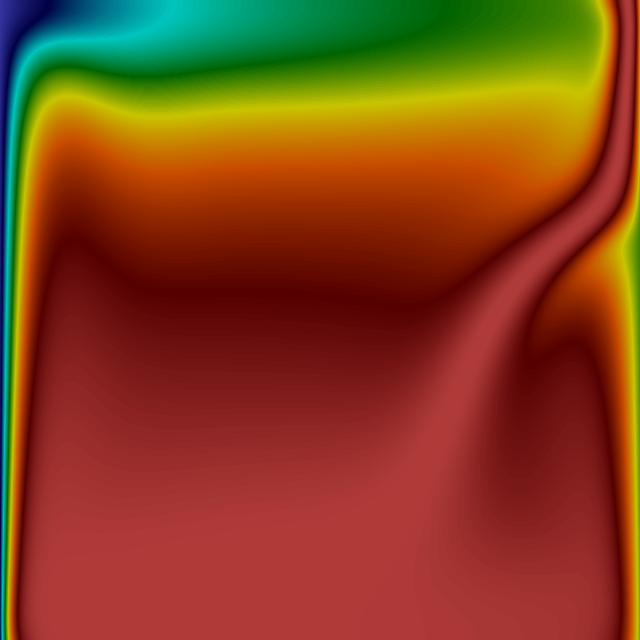
\includegraphics[width=.25\linewidth]{rho_750s_CF.png} &  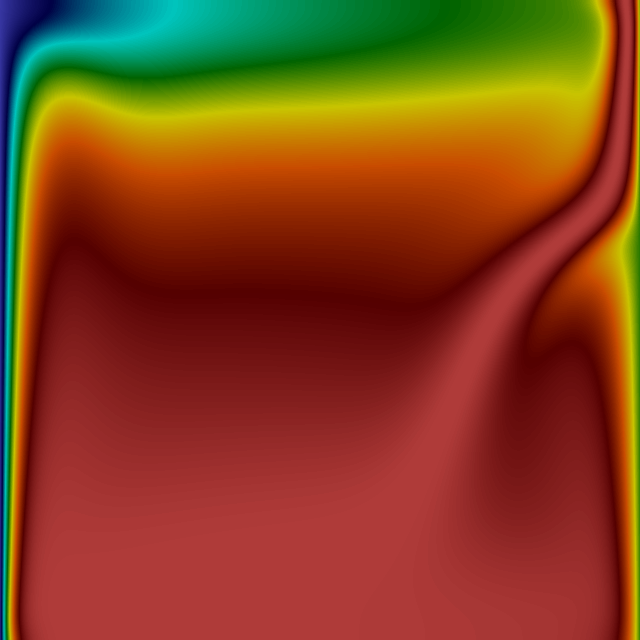
\includegraphics[width=.25\linewidth]{CF_rho_1500s.png} & 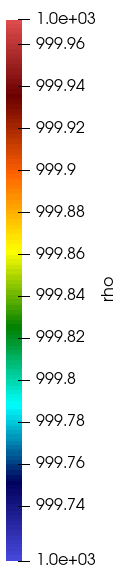
\includegraphics[width=.0558\linewidth]{rho.png} \\ \bottomrule[1pt]		
	\end{tabular}
	\centering
	\caption{Numerical results of Natural convection modified solver between \textit{t = 750s} and \textit{1500s}.}	
	\label{3.7tab}
\end{table}

\clearpage
\section{OpenFOAM: IcoReactingMultiphaseInterFOAM. Phase-Change Process}
\setlength{\parindent}{0.5cm} The solidification process is assessed in this section with two elaborated models. Both of the models are implemented within a multi-phase solver based on the volume of fluid technique. This technique aims to capture interface and enhances contact angle and surface tension for each phase. Thus, the first model is based on the coupling of the VOF and the enthalpy-porosity method. To accomplish the inclusion of the enthalpy-porosity method, a library in which the latent heat is implemented as an explicit source term for the energy equation in the solver. 

\noindent On the other hand, the second model uses the VOF method combined with a semi-empirical model based on the work of Lee. The empirical constant is adapted here to be used in conjunction with the use of the \textit{Classical Nucleation Theory}.

\section{Case Description.}

\setlength{\parindent}{0.5cm} Two regular geomtries are created: a squared cavity, used in the pure convection case and a cylindrical plane geometry. Both geometries test both solidification models.

\begin{figure}[h!]
	\centering
	\begin{subfigure}{\linewidth}
		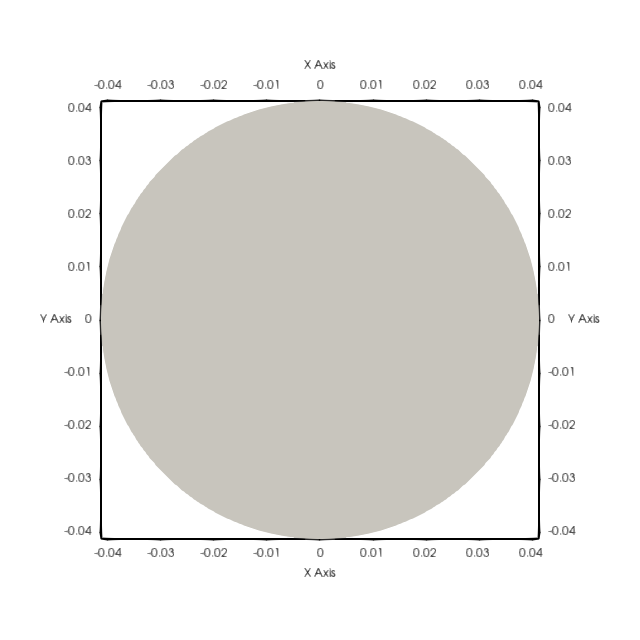
\includegraphics[width=.55\linewidth]{cylinder_geom.png}\hfill
		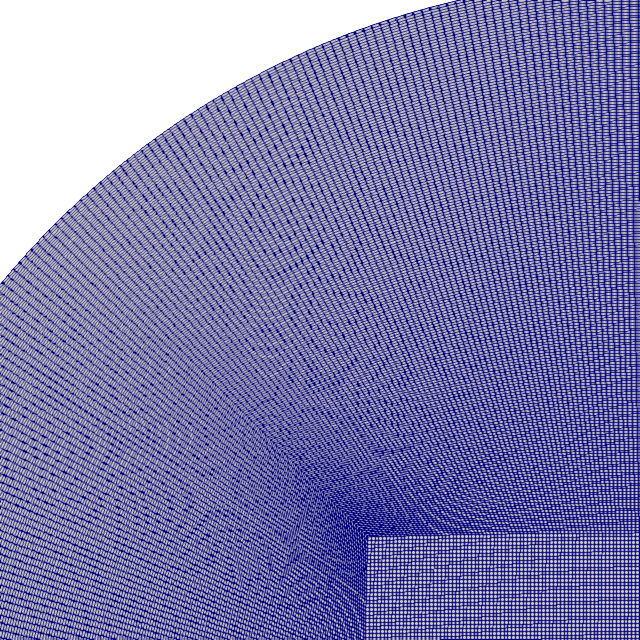
\includegraphics[width=.35\linewidth]{mesh_cylinder.png}	
		\label{BBPF_NCMF}
	\end{subfigure}
	\label{3.7fig}
	\caption{Geometric characteristics for cylinder.}
\end{figure} 
The computed structured mesh consists of 572404 nodes.

\subsection{Hypotheses And Assumptions}

\setlength{\parindent}{0.5cm} To carry out the phase-transition process, some assumptions are taken into account so as to simplify the multiphysics ocurring during such arising phenomena. 

\textbf{Laminar regime:} The Reynolds number, computed from the maximum velocity is not high enough to consider turbulent effects. 

\noindent In the current case-scenario, a Prandtl close to 7. 

\textbf{Newtonian fluid:} The viscosity of the fluid is assumed to be constant.
The thermophysical properties treatment is described below.

\textbf{Quasy-steady state:} Bourdillon \cite{bourdillon_2016} used the hypothesis of quasy-steady solution of the natural convective solver as initial condition in the solidification process. As many researchers as Yan et al. \cite{yan_xu_qiu_gang_2017} suggest, water presents a high latent heat of solidification when the heat released during freezing plays a greater role than the transient process of heat accumulation in the layer of the phase being developed. In other words, when the latent heat of the phase change material is larger than its sensible heat, the latter is having little influence on the temperature distribution of the PCM. In such case, the interface is moving slowly and the temperature distribution, at a given time step, keeps constant. Therefore, for comparison purposes against literature results, the solidification process in a cavity is tested using a quasy-steady solution obtained in the pure convection case.

\subsubsection*{Two phase properties}
\setlength{\parindent}{0.5cm} Within a multiphase framework, a model reflects a jump in properties through the interphase. Thus, a smooth transition between phase properties must be achieved.
\begin{equation}
	\lambda=\lambda_{\ell} \alpha_{\ell}+\lambda_{s} f_{s}
	\label{3.35}
\end{equation}
\begin{equation}
	C_{p}=C_{p_{\ell}} \alpha_{\ell}+C_{p_{s}} f_{s}
	\label{3.36}
\end{equation}
\begin{equation}
	\mu=\mu_{\ell} \alpha_{\ell}+\mu_{s} f_{s}
	\label{3.37}
\end{equation}
In the current case-scenario, $C_{p_{s}}=C_{p_{l}}$.

\noindent In the case of polynomial density variation it is settled in a similar manner. The polynomial is not thought to suit negative temperatures, and when the problem is within this range, the density should take ice's density.
\begin{equation}
	\rho(T)^{\prime}=\rho(T) \alpha_{\ell}+\rho_{s} \alpha_{s}
	\label{3.38}
\end{equation}
where $\alpha_{l}$ and $\alpha_{s}$ are liquid and solid volume fractions, respectively.		
\subsection{Governing Equations}

\setlength{\parindent}{0.5cm} This section is devoted to describe the governing equations that the solidification process requires. Beside the presented conservation equation for the volume of fraction needed for the VOF method, Eq. \ref{VOFEQ},
\begin{equation}
	\frac{\partial \alpha_{\text {phase }}}{\partial t}+\frac{\partial\left(\alpha_{\text {phase }} u_{j}\right)}{\partial x_{j}}=0
	\label{VOFEQ}
\end{equation}
in the next sections, momentum and energy equations are revisited.

\subsubsection{Momentum Equation}

\setlength{\parindent}{0.5cm} The momentum equation has the same terms as per each one of the models. Here it is the equation recalled from previous section:
\begin{equation}
	\label{3.39}
	\begin{aligned}
	&\frac{\partial\left(\rho {u}_{i}\right)}{\partial t}+\frac{\partial\left(\rho {u}_{i} {u}_{j}\right)}{\partial x_{j}} \\
	&\quad=-\alpha_{i} \nabla p+\frac{\partial}{\partial x_{j}}\left(\mu \frac{\partial {u}_{i}}{\partial x_{j}}\right)+F_{\sigma i}+S_{u_{i}}
	\end{aligned}
\end{equation}

\subsubsection{Energy Equation}

\setlength{\parindent}{0.5cm} On the other side, the energy equation slightly differs from one model to the other. As pointed out before, here there are recalled both energy equations.
The energy equation for the Enthalpy-porosity model:
\begin{equation}
\begin{aligned}
\frac{\partial (\rho C_{p} T)}{\partial t}+ \nabla \cdot\left(u_{j}\rho C_{p} T\right)+L\left[\frac{\partial (\rho \alpha_{l}\gamma_{l})}{\partial t}+ \frac{\partial (u_{j}\rho \alpha_{l}\gamma_{l})}{\partial x_{j}}\right]=\nabla \cdot\left(k_{i} \nabla T_{i}\right)
\end{aligned}
\label{3.40}
\end{equation}
The energy equation for the Lee model in conjunction with the nucleation theory:
\begin{equation}
\label{3.41}
\frac{\partial (\rho C_{p} T)}{\partial t}+\nabla \cdot\left(u_{j}\rho C_{p} T\right)=\nabla \cdot\left(k_{i} \nabla T_{i}\right)+S_{H_{i}}
\end{equation}

\subsection{Solver description. Control Loop}

\setlength{\parindent}{0.5cm} IcoReactingMultiphaseInterFoam solver is a multiphase, multicomponent incompressible solver based on volume of fluid method. The solver captures the interfaces and includes contact angle and surface tension effects for each phase. Moreover, this solver supports mass and heat transfer across phases.

\subsection{Mass transfer models}
For each pair of phases, two mass transfer models might be used:
\begin{itemize}
	\item \textbf{Lee model:} Used for solid melting and liquid solidification.
	\item \textbf{KineticGasEvaporation:} Used for condensation and evaporation.
\end{itemize}
In this thesis, only the Lee model will be considered for further explanation.


\subsection{Code implementations}

\setlength{\parindent}{0.5cm} Within the entalphy-porosity model, the source term belonging to the calculation of the latent heat is added within the OpenFOAM framework. The energy equation of the solver shown in Eq. \ref{3.41} is thereby implemented in Fig. \ref{3.8fig}
\begin{figure}[h!]
	\centering
	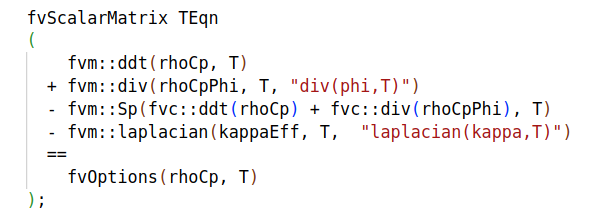
\includegraphics[width=0.6\linewidth]{TEqn.png}\hfill	
	\caption{Energy equation of IcoReactingMultiphaseInterFoam.}
	\label{3.8fig}
\end{figure}
In the term belonging to the RHS of the equation, the solver calls the implemented library \textit{mySolidificationMeltingSource} that calculates the latent heat source term as it appears in the figure \ref{3.9fig}:
\begin{figure}[h!]
	\centering
	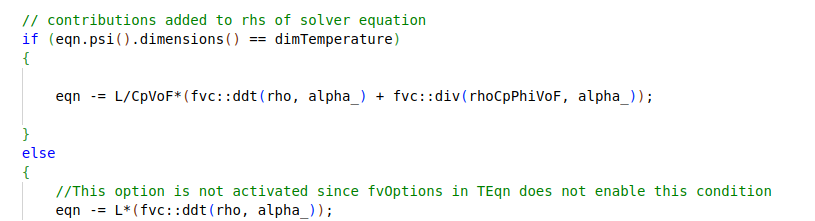
\includegraphics[width=0.8\linewidth]{solidification_latent_heat.png}\hfill
	\caption{Latent heat source term present in mySolidificationMeltingSource library.}
	\label{3.9fig}
\end{figure}

\noindent Here, the alpha variable showing up in the calculation is obtained through a linear expression that gives the amount of energy contained in the fluid cell above the melting point. This is divided by the latent heat to obtain the liquid fraction. Then, this fraction is constained between 0 and 1. Further details on the code can be found in \ref{Enthalpy-porosity library}. The liquid fraction is calculated instead of being obtained through the transport equation worked out within the VOF method so it can be used in other solvers. This is explained later in this thesis.

The \textbf{rhoCpPhiVoF} term, which is called in this library, is created in \textit{createFields.H} as a variable field so that it can be called from everywhere within the code.
\clearpage
\begin{figure}[h!]
	\centering
	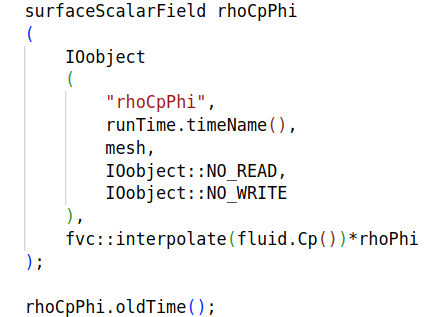
\includegraphics[width=0.4\linewidth]{rhocpphicreate.png}\hfill	
	\caption{\textbf{rhoCpPhi} field in \textit{createFields.H}}
	\label{3.10fig}
\end{figure}
 
\noindent The implemented library can be found in the Appendix \ref{AppendixA}, section \ref{Enthalpy-porosity library}. 

\noindent On the core of the other model, the basis of the Lee model is already implemented in OpenFOAM. However, there is a parameter, \textit{C}, devoted to act as a condensation rate. This is referred as an empirical coefficient used to speed-up or slow down the mass and heat transfer. The physics behind are unknown for this solver, therefore, in favor of tunning this parameter in accordance with the characteristic behavior of the water when it freezes, the \textit{Classical Nucleation theory} is followed.
\newline
\begin{figure}[h!]
	\centering
	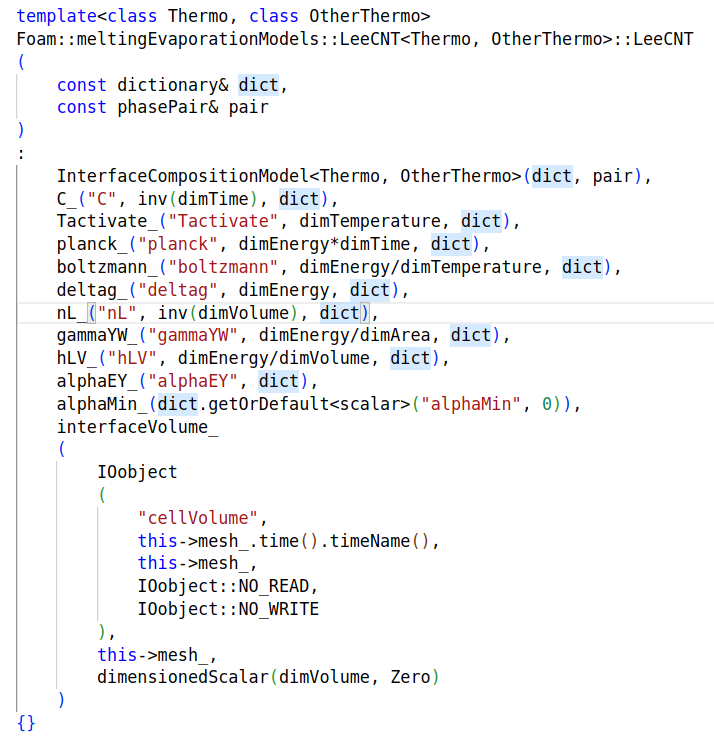
\includegraphics[width=0.6\linewidth]{LeeCNT.png}\hfill	
	\caption{Library function in LeeCNT.}
	\label{3.11fig}
\end{figure}
\newline
In the function shown above, all of the parameters concerning the formulas required to calculate the nucleation rate of the water are user-defined parameters except for the \textbf{cellVolume} which is an implicit function that calculates the volume per each cell. In the Appendix \ref{AppendixA}, the code related with the Lee model using this theory can be found.

\subsection{Case Setup}
\subsubsection*{Boundary conditions}

For the squared cavity:
The initial conditions for the internal field of the cavity regarding the velocity, temperature and pressure magnitudes are inherited from the last timestep of the natural convection case under the assumption of quasi-steady state. The temperature of the right wall is suddenly decreased to 263K.

\begin{table}[h!]
	\begin{tabular}{@{}lllll@{}}
		\toprule[1pt]
		\textbf{Boundary} & \textbf{Conditions}  \\ \midrule[2pt]
		Left & $T_{l}=283, v_{l} = 0, \frac{\partial \alpha_{l}}{\partial n} = 0, \frac{\partial \alpha_{s}}{\partial n} = 0    $  \\
		Right & $T_{r}=263, v_{r} = 0, \alpha_{l} = 1, \alpha_{s} = 0 $ \\
		Upper & $\frac{\partial T_{u}}{\partial n} = 0, v_{u} = 0, \frac{\partial \alpha_{l}}{\partial n} = 0, \frac{\partial \alpha_{s}}{\partial n} = 0$  \\
		Bottom & $\frac{\partial T_{b}}{\partial n} = 0, v_{b} = 0, \frac{\partial \alpha_{l}}{\partial n} = 0, \frac{\partial \alpha_{s}}{\partial n} = 0 $  \\ \bottomrule[1pt]		
	\end{tabular}
	\centering
	\caption{Boundary conditions for natural convection case. Cavity case.}	
	\label{3.8tab}
\end{table}

\noindent frontAndBack boundary is set to \textit{empty} to define a 2-dimensional case-scenario. 

For the cylinder:
\begin{table}[h!]
	\begin{tabular}{@{}lllll@{}}
		\toprule[1pt]
		\textbf{Boundary} & \textbf{Conditions}  \\ \midrule[2pt]
		Walls & $T=255, v = 0,\frac{\partial \alpha_{l}}{\partial n} = 0, \frac{\partial \alpha_{s}}{\partial n} = 0    $  \\
		Internal field & $T=294, v = 0, \alpha_{l} = 1, \alpha_{s} = 0 $ \\
		\bottomrule[1pt]		
	\end{tabular}
	\centering
	\caption{Boundary conditions for natural convection case. Cylinder case.}	
	\label{3.9tab}
\end{table}

\noindent As in the previous geometry, there is an empty boundary called frontAndBack to define a planar case.

\noindent The thermophysical properties and solver parameters defined below are setted up for both geometries.
\clearpage
\subsubsection*{Thermophysical properties}
\begin{table}[h!]
	\begin{tabular}{@{}lllll@{}}
		\toprule[1pt]
		\textbf{Water properties} & \textbf{Symbol} & \textbf{Values} & \textbf{Units} &  \\ \midrule[2pt]
		Water density & $\rho_l$ & 999.8 & $kg.m^{-3}$ \\
		Ice density & $\rho_s$ & 916.8 & $kg.m^{-3}$ \\		
		Water kinematic viscosity & $\nu_{l}$ & 1.79e-6 & $m^{2}.s^{-1}$ \\
		Ice kinematic viscosity & $\nu_{s}$ & 2.0e-6 & $m^{2}.s^{-1}$ \\		
		Water thermal conductivity & $\lambda_{l}$ & 0.56 & $W.m^{-1}.K^{-1}$ \\
		Ice thermal conductivity & $\lambda_{s}$ & 2.26 & $W.m^{-1}.K^{-1}$ \\		
		Heat capacity & $C_{p_{l}}=C_{p_{s}}$ & 4202 & $J.kg.K^{-1}$ \\		 
		Gravitational acceleration & $g$ &  9.81  & $m.s^{-2}$ \\
		Thermal diffusivity & $\gamma$ &  1.435e-7  & $m^{2}.s^{-1}$ \\		
		Thermal expansion coefficient & $\beta$ &  6.734e-5  & $K^{-1}$ \\
		Latent heat & $L$ &  335000  & $J.K^{-1}$ \\			
		Laminar Prandtl number & $P_r$ &  6.99  & - \\
		Reference temperature & $T_r$ &  6.734e-5  & $K$ \\
		Darcy's constant & $D_c$ &  10e8  & - \\		 \bottomrule[1pt]		
	\end{tabular}
	\centering
	\caption{Water properties for natural convection.}	
	\label{3.10tab}
\end{table}
In table \ref{3.11tab} are detailed the parameters used in the implemented nucleation library for the Lee model.
\begin{table}[h!]
	\begin{tabular}{@{}lllll@{}}
		\toprule[1pt]
		\textbf{Water nucleation properties} & \textbf{Symbol} & \textbf{Values} & \textbf{Units} &  \\ \midrule[2pt]
		Planck constant & $h$ & 6.63e-34 & $J.s$ \\
		Boltzmann constant & $k_{B}$ & 1.38e-23 & $J.K^{-1}$ \\		
		Gibbs free energy & $\Delta_{gv}$ & 4e-20 & $J$ \\
		Interfacial tension & $\gamma_{yw}$ & 2.91e-2 & $J.m^{-2}$ \\		
		Latent heat per volume & $H_{lv}$ & 3.10e8 & $J.m^{-3}$ \\
		Shape coefficient of nucleation & $\alpha_{ey}$ & 0.0001 & - \\		
		Water molecule per volume & $n_{L}$ &  5.5e4  & $m^{3}$ \\		 \bottomrule[1pt]		
	\end{tabular}
	\centering
	\caption{Water properties for solidification.}	
	\label{3.11tab}
\end{table}
The solver parameters used for the discretization of the different terms in the equations are pointed out next. 

\subsubsection*{Solver parameters}
So as to obtain a minimum expected accuracy during the calculation, in table \ref{3.13tab} are the chosen parameters for the equation solvers.
\clearpage
\begin{table}[h!]
\begin{adjustbox}{width=1\textwidth}
	\small		
	\begin{tabular}{@{}lllll@{}}
		\toprule[1pt]
		\textbf{Equation} & \textbf{Linear Solver} & \textbf{Smoother/Preconditioner} & \textbf{Tolerance} &  \\ \midrule[2pt]
		Pressure correction equation (P) & PCG & DIC & 1e-5 \\
		Momentum equation (U)& smoothSolver & symGaussSeidel  & 1e-06 \\
		Volume fraction equation (alpha) & smoothSolver & symGaussSeidel  & 1e-8 \\
		Species equation  (Y)   & smoothSolver   & symGaussSeidel &1e-09 \\		 
		Energy equation (T)    &  PBiCG  &  DILU
		&  1e-08  \\ \bottomrule[1pt]		
	\end{tabular}
\end{adjustbox}
	\centering
	\caption{Solvers for the discretised equations.}	
	\label{3.13tab}
\end{table}
\clearpage
\subsection{Validation of Results and Conclusions}
\label{Convection-case}
\setlength{\parindent}{0.5cm} The validation of the phase change problem is achieved by different methodologies. First, the enthalpy-porosity and Lee-CNT models are compared with available data found in the doctoral thesis of Borudillon \cite{bourdillon_2016} and the experimental data of Kowalewski et al. \cite{kowalewski_rebow_1999}. And later, the Lee-CNT model is tested against the classical Stefan problem.

\noindent So as to understand the physical phenomena underlaying these plots, a first general explanation is given. 

\noindent In figure \ref{3.13figa}, temperature distribution along x mid-plane shows a first sudden decrease whithin the initial position and $x < 0.2$ due to the existing temperature gradient between the left wall and the internal field temperature obtained from the quasi-steady solution in the natural convection solver. After that, nearly $0.1 \leq x \leq 0.2$, and induced by the upper clockwise recirculation, the temperature along this mid-plane and until $x \approx 0.6$, is submitted to an increase. From there on, the existence of two colliding and opposite recirculating flows induce a second decrease of the temperature which lasts until $x \approx 0.9$. Then, the influence of the proximity with the cold wall makes the temperature dimensionless to undergo a fast decrease.

\noindent If one recalls now in the temperature distribution along the vertical mid-plane, Fig. \ref{3.13figb}, it is depicted how the temperature increases slowly at the bottom of the cavity $0 \leq y \leq 0.2$. This is mainly due to the gravity related terms which determine the buoyancy effects within the domain. Thereafter, when in the range of $0.2 \leq y \leq 0.4$ there is an increase speed-up by the effects of the recirculating flows colliding with each other. From $y \approx 0.4$ towards the top of the cavity, the recirculating flow induces a slowly increase in the temperature.

\noindent Moving along the U-velocity dimensionless component, ,Fig. \ref{3.13figc}, a first oscillation is observed near the left wall at $x \approx 0.1$. Then, at $0.6 \leq x \leq 0.8$, it shows up a sudden decrease in the velocity magnitude due the clockwise direction that the upper flow exhibits as long as the ice layer formation advances in time. From $0.7 \leq x \leq 1$ the velocity component increases rapidly until it reaches a 0 constant value due to the appearence of the solid ice layer. 

\noindent Describing the U-velocity profile along the vertical line, Fig. \ref{3.13figd}, one sees how the first negative peak in $0.2 \leq y \leq 0.3$ is highly influenced by the effect of the counter clockwise lower recirculating flow generated by the upper flow (rotating clockwise) when interacts with the ice layer advancing front. Moving up along the vertical line, the behavior of the velocity component tends to increase since it starts being influenced by the upper recirculating flow, in $0.3 \leq y  \leq 0.9$, and until it reaches a 0 value induced by the adiabatic and the zero gradient velocity condition applied in top and bottom walls.

\noindent Similarly, the V-velocity along the x mid-plane, Fig. \ref{3.13figc}, displays a peak near the left wall where the direction of the upper flow is clockwise. As one moves farther from the left wall, the velocity components are not constituted yet. Comparatively as with the U-velocity along the x mid-plane, the influence of the lower recirculating flow brings negative dimensionless velocity vectors in the vertical magnitudes. This is in the region where $0.6 \leq x \leq 0.7$. At $0.75 \leq x \leq 0.8$ the recirculating flows in this region slightly influences the increase of the velocity. From there on, the velocity gets reduced until it reaches a zero constant value due to the sink of velocity magnitude in the ice layer zone.

\noindent Finally, the V-velocity plotted along the y mid-plane depicts a negative peak at $y \approx 0.3$. This is mainly influenced by the negative dimensionless velocity values arising from the recirculating flow taking place from the collision of the upper flow and the ice layer.

\begin{table}[h!]
	\begin{tabular}{@{}b{2cm}ccc@{}}
		\toprule[1pt]
		& 
		\multicolumn{1}{c}{\textbf{Lee model-CNT}} & \\ \midrule[2pt]
		\vbox to 3\baselineskip{\textbf{Temperature}}& 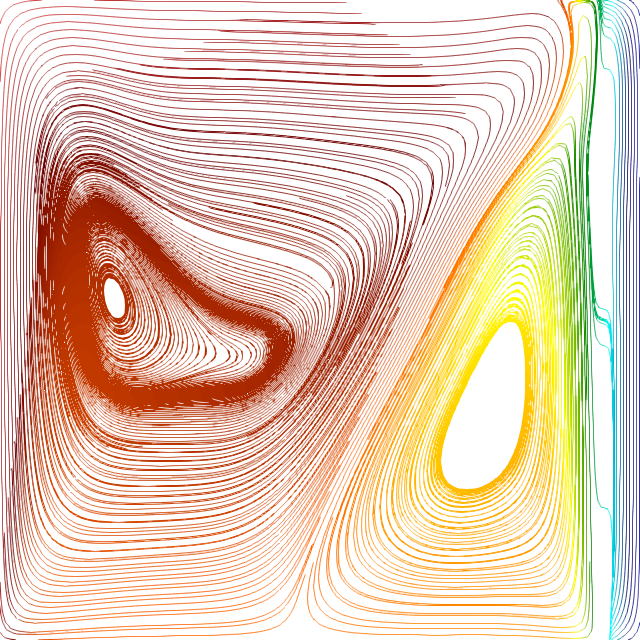
\includegraphics[width=.25\linewidth]{t_x_streamlines.png} & 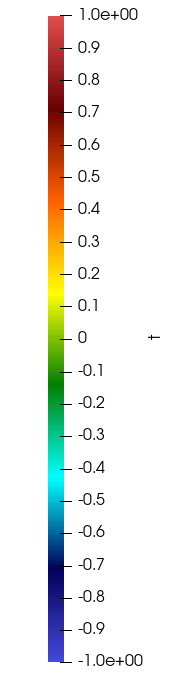
\includegraphics[width=0.078\linewidth]{t_x_scale.png} \\		
		\vbox to 3\baselineskip{\textbf{U-velocity}}&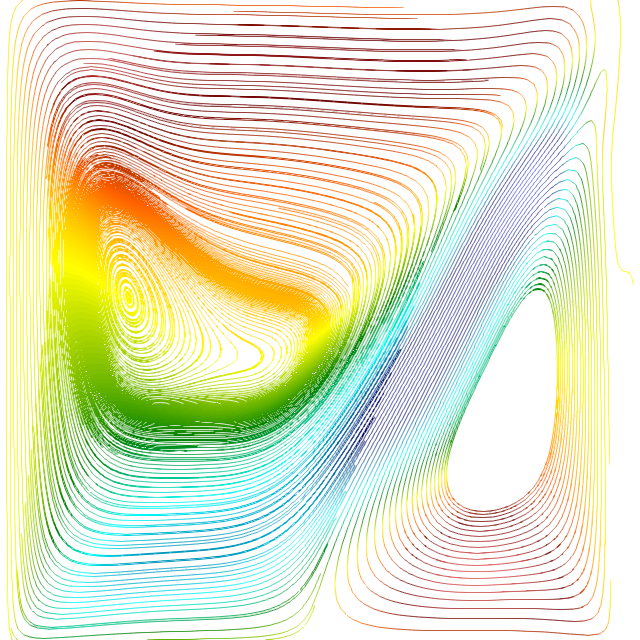
\includegraphics[width=.25\linewidth]{u_x_streamlines.png} & 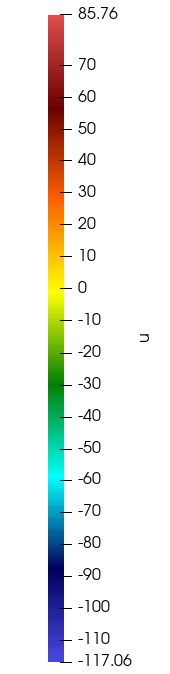
\includegraphics[width=0.078\linewidth]{u_x_scale.png}\\
		\vbox to 3\baselineskip{\textbf{V-velocity}}& 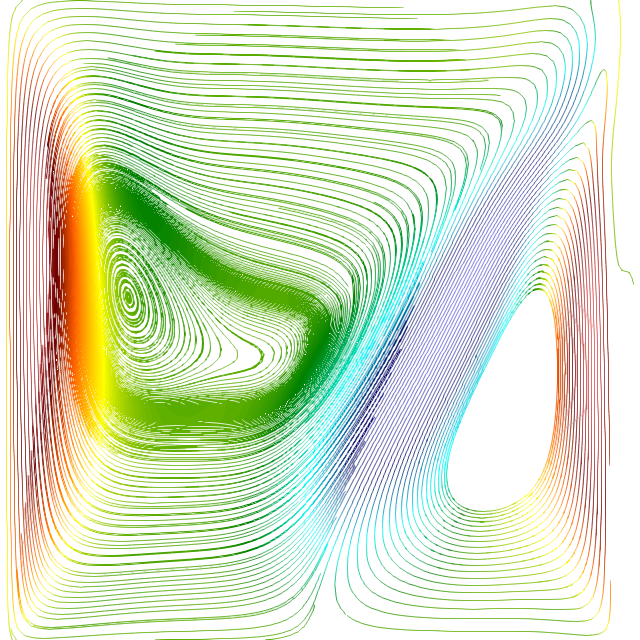
\includegraphics[width=.25\linewidth]{v_x_streamlines.png} & 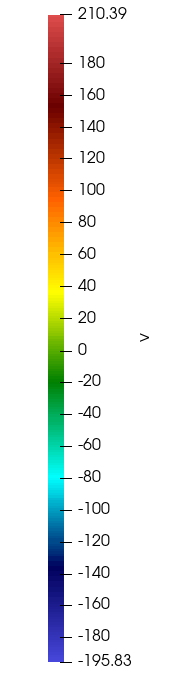
\includegraphics[width=0.078\linewidth]{v_x_scale.png} \\	 \bottomrule[1pt]		
	\end{tabular}
	\centering
	\caption{Numerical results of dimensionless magnitudes for Lee-CNT model at \textit{t = 100s}.}	
	\label{3.15tab}
\end{table}


\begin{figure}[h!]
	\begin{subfigure}{0.50\textwidth}
		\centering
		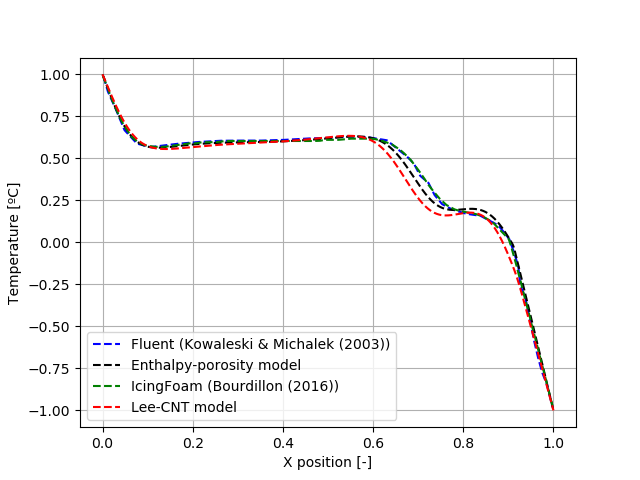
\includegraphics[width=\linewidth]{T_xpos_cavity_comparative.png}\hfill
		\caption{Temperature along horizontal line.} \label{3.13figa}
	\end{subfigure}
	\hfill
	\begin{subfigure}{0.50\textwidth}
		\centering
		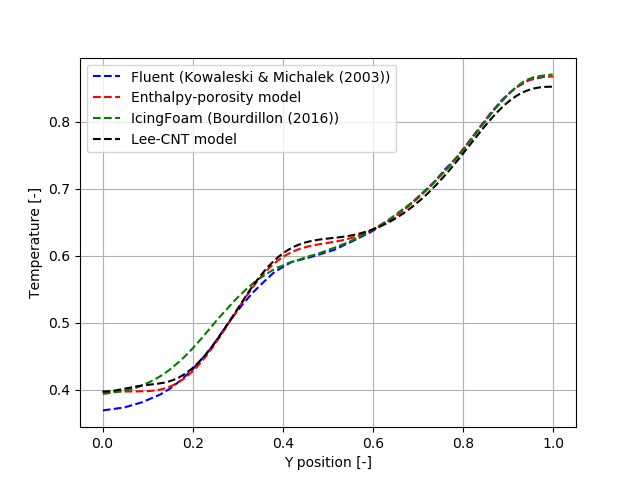
\includegraphics[width=\linewidth]{T_ypos_cavity_comparative.png}	
		\caption{Temperature along vertical line.}\label{3.13figb}
	\end{subfigure}
	\begin{subfigure}{0.50\textwidth}
		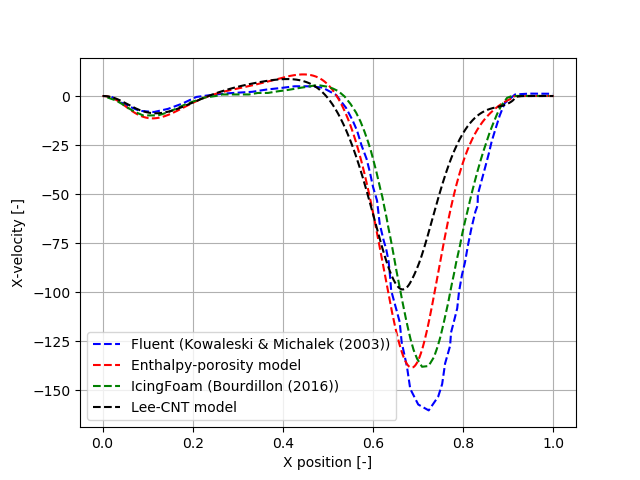
\includegraphics[width=\linewidth]{xvel_xpos_cavity_comparative.png}\hfill
		\caption{U-velocity along horizontal line.}\label{3.13figc}
	\end{subfigure}
	\begin{subfigure}{0.50\textwidth}
		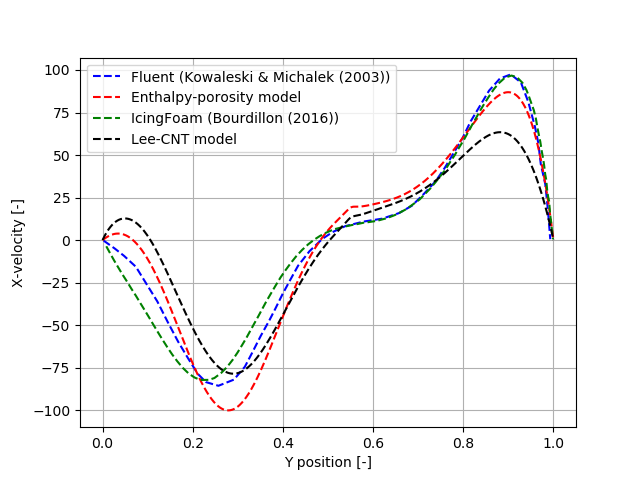
\includegraphics[width=\linewidth]{xvel_ypos_cavity_comparative.png}	
		\caption{U-velocity along vertical line.}\label{3.13figd}
	\end{subfigure}
	\begin{subfigure}{0.50\textwidth}
		\includegraphics[width=\linewidth]{yvel_xpos_cavity_comparative.png}\hfill	
		\caption{V-velocity along horizontal line.}\label{3.13fige}
	\end{subfigure}
	\begin{subfigure}{0.50\textwidth}
		\includegraphics[width=\linewidth]{yvel_ypos_cavity_comparative.png}	
		\caption{V-velocity along vertical line.}\label{3.13figf}
	\end{subfigure}
	\caption{Adimensional magnitudes comparison at \textit{t = 100s}.}
	\label{3.13fig}
\end{figure}
\clearpage
\noindent Dimensionless quantities presented in the section \ref{Convection-case} are here discussed for solidification comparison purposes. Temperature dimensionless results for the Enthalpy-porosity and Lee-CNT models are in a good agreement with Fluent and IcingFoam results. However, large discrepancies arise in the evolution of the velocity magnitudes. With special mention to U-velocity along x mid-plane, \ref{3.13figc} and V-velocity along y mid-plane, \ref{3.13figf}. Comparatively, the Enthalpy-porosity model tends to overpredict the velocity magnitude with respect to the Lee-CNT model and therefore it predicts a faster formation of a well-developed shape front. The results also show a minimal shift between numerical solutions due to the advancing front which tends to slightly infer in the evolution of the physical magnitudes.

\begin{table}[h!]
	\begin{tabular}{@{}b{2cm}ccc@{}}
		\toprule[1pt]
		 & 
		\multicolumn{1}{c}{\textbf{Enthalpy-porosity}} & \multicolumn{1}{c}{\textbf{Lee model-CNT}} \\ \midrule[2pt]
		\vbox to 3\baselineskip{\textbf{T=100s}}& \includegraphics[width=.25\linewidth]{T_1600s_EP_cavity.png} & \includegraphics[width=.25\linewidth]{T_1600s_CNT_cavity.png} &
		\includegraphics[width=.0658\linewidth]{T_scale_EP_cavity.png} \\		
		\vbox to 3\baselineskip{\textbf{T=200s}}&\includegraphics[width=.25\linewidth]{T_1700s_EP_cavity.png} & \includegraphics[width=.25\linewidth]{T_1700s_CNT_cavity.png} &  \includegraphics[width=.0658\linewidth]{T_scale_EP_cavity.png} \\
		\vbox to 3\baselineskip{\textbf{T=300s}}& \includegraphics[width=.25\linewidth]{T_1800s_EP_cavity.png} & \includegraphics[width=.25\linewidth]{T_1800s_CNT_cavity.png} &
		\includegraphics[width=.0658\linewidth]{T_scale_EP_cavity.png} \\	 \bottomrule[1pt]		
	\end{tabular}
	\centering
	\caption{Numerical results of temperature distributions for Enthalpy-porosity and Lee-CNT models at \textit{t = 100, 200, 300s}.}	
	\label{3.15tab}
\end{table}
\clearpage

\begin{table}[h!]
	\begin{tabular}{@{}b{2cm}ccc@{}}
		\toprule[1pt]
		& 
		\multicolumn{1}{c}{\textbf{Enthalpy-porosity}} & \multicolumn{1}{c}{\textbf{Lee model-CNT}} \\ \midrule[2pt]
		\vbox to 3\baselineskip{\textbf{T=100s}}& \includegraphics[width=.25\linewidth]{U_1600s_EP_cavity.png} & \includegraphics[width=.25\linewidth]{U_1600s_CNT_cavity.png} &
		\includegraphics[width=.0658\linewidth]{U_scale_1600s_cavity.png} \\		
		\vbox to 3\baselineskip{\textbf{T=200s}}&\includegraphics[width=.25\linewidth]{U_1700s_EP_cavity.png} & \includegraphics[width=.25\linewidth]{U_1700s_CNT_cavity.png} &  \includegraphics[width=.0658\linewidth]{U_scale_1700s_cavity.png} \\
		\vbox to 3\baselineskip{\textbf{T=300s}}& \includegraphics[width=.25\linewidth]{U_1800s_EP_cavity.png} & \includegraphics[width=.25\linewidth]{U_1800s_CNT_cavity.png} &
		\includegraphics[width=.0658\linewidth]{U_scale_1800s_cavity.png} \\	 \bottomrule[1pt]		
	\end{tabular}
	\centering
	\caption{Numerical results of velocity distributions for Enthalpy-porosity and Lee-CNT models at \textit{t = 100, 200, 300s}.}	
	\label{3.16tab}
\end{table}
\noindent In the figures shown in the tables \ref{3.15tab}, \ref{3.16tab}, and \ref{3.17tab} are depicted the main physical phenomena of the solidification process. Temperature fields, velocity magnitudes and liquid volume fraction are chosen in order to visually detect the minimum local differences as the phase change gets more developed. As commented above, and shown in table \ref{3.16tab}, the Enthalpy-porosity model overpredicts the velocity magnitude until the extent of exhibiting a well-developed "belly" shape front. Contrarily, the evolution of the velocity magnitude in the Lee-model is under-predicted in comparison with the Enthalpy-porosity model, fact that leads to a more planar shape of the advancing ice layer.
\clearpage
\begin{table}[h!]
	\begin{tabular}{@{}b{2cm}ccc@{}}
		\toprule[1pt]
		& 
		\multicolumn{1}{c}{\textbf{Enthalpy-porosity}} & \multicolumn{1}{c}{\textbf{Lee model-CNT}} \\ \midrule[2pt]
		\vbox to 3\baselineskip{\textbf{T=100s}}& \includegraphics[width=.25\linewidth]{alpha_1600s_EP_cavity.png} & \includegraphics[width=.25\linewidth]{alpha_1600s_CNT_cavity.png} &
		\includegraphics[width=.0658\linewidth]{alpha_scale_cavity.png} \\		
		\vbox to 3\baselineskip{\textbf{T=200s}}&\includegraphics[width=.25\linewidth]{alpha_1700s_EP_cavity.png} & \includegraphics[width=.25\linewidth]{alpha_1700s_CNT_cavity.png} &  \includegraphics[width=.0658\linewidth]{alpha_scale_cavity.png} \\
		\vbox to 3\baselineskip{\textbf{T=300s}}& \includegraphics[width=.25\linewidth]{alpha_1800s_EP_cavity.png} & \includegraphics[width=.25\linewidth]{alpha_1800s_CNT_cavity.png} &
		\includegraphics[width=.0658\linewidth]{alpha_scale_cavity.png} \\	 \bottomrule[1pt]		
	\end{tabular}
	\centering
	\caption{Numerical results of fluid fraction distributions for Enthalpy-porosity and Lee-CNT models at \textit{t = 100, 200, 300s}.}	
	\label{3.17tab}
\end{table}
\noindent In the next figures, simulations have been carried out with a cylindrical geometry for a physical time of \textit{5000s}. Initially good agreement between Lee-CNT and Enthalpy-porosity models compared with Fluent and IcingFoam. As results in table \ref{3.18} show, the evolution of temperature, velocity and liquid fraction magnitudes are quite similar, however, one might appreciate slight differences in the velocity magnitudes from \textit{t = 100s} to \textit{300s}. This will be further commented below.
\clearpage
\begin{table}[h!]
	\begin{tabular}{@{}b{2cm}lll@{}}
		\toprule[1pt]
		&\multicolumn{1}{c}{\textbf{Enthalpy-porosity}} & 
 		\multicolumn{1}{c}{\textbf{Lee model-CNT}} \\ \midrule[2pt]
		\vbox to 3\baselineskip{\textbf{T=100s}}&\includegraphics[width=.25\linewidth]{T_100s_EP.png} & \includegraphics[width=.25\linewidth]{T_100s_CNT.png} &
		\includegraphics[width=.0658\linewidth]{T_scale_100s_EP.png} \\
		\vbox to 3\baselineskip{\textbf{T=300s}}&\includegraphics[width=.25\linewidth]{T_300s_EP.png} &
		\includegraphics[width=.25\linewidth]{T_300s_CNT.png} & 
		\includegraphics[width=.0658\linewidth]{T_scale_300s_EP.png} \\
		\vbox to 3\baselineskip{\textbf{T=100s}}& \includegraphics[width=.25\linewidth]{U_100s_EP.png} & \includegraphics[width=.25\linewidth]{U_100s_CNT.png} &  \includegraphics[width=.0558\linewidth]{U_scale_100s_EP.png} \\
		\vbox to 3\baselineskip{\textbf{T=300s}}& \includegraphics[width=.25\linewidth]{U_300s_EP.png} & \includegraphics[width=.25\linewidth]{U_300s_CNT.png} &  \includegraphics[width=.0558\linewidth]{U_scale_300s_EP.png} \\
		\vbox to 3\baselineskip{\textbf{T=100s}}&\includegraphics[width=.25\linewidth]{alpha_100s_EP.png} & \includegraphics[width=.25\linewidth]{alpha_100s_CNT.png} &  \includegraphics[width=.0558\linewidth]{alpha_scale_cavity.png} \\
		\vbox to 3\baselineskip{\textbf{T=300s}}&\includegraphics[width=.25\linewidth]{alpha_300s_EP.png} & \includegraphics[width=.25\linewidth]{alpha_300s_CNT.png} &  \includegraphics[width=.0558\linewidth]{alpha_scale_cavity.png} \\ \bottomrule[1pt]		
	\end{tabular}
	\centering
	\caption{Numerical results of Enthalpy-porosity and Lee-CNT models at \textit{t = 100s} and \textit{300s} in a cylinder.}	
	\label{3.18tab}
\end{table}
\clearpage
Here in Fig. \ref{zoomInterface} it is shown the description of the interface. There it can be checked the mushy region where the liquid fraction is $0 < \alpha_{l} < 1$.
\begin{figure}[h!]
	\centering
	\includegraphics[width=.3\linewidth]{alpha_zoom.png}	
	\caption{Gradient of the interface between liquid and solid phases for Lee-CNT model.}
	\label{zoomInterface}
\end{figure} 

\noindent In the figure \ref{3.12fig}, temperature magnitude is in the center of the cylinder along time. Here, it can be appreciated three different zones: for $0s < t < 400s$, it belongs to the convection heat transfer period, then, for $400s < t < 4000s$ there exists a mushy zone, the water is loosing heat by this time. For $t > 4000s$ solidification begins. As it might be observed in \ref{3.12fig}, but also in the temperature distribution at \textit{t=300s} in table \ref{3.18}, near $300s < t < 600s$ the effect of the density inversion begins to be visible at $T \approx 5 \deg C$. As it happened for the cavity case, the fact of characterizing the density with a polynomial function allows the solver to see a phenomena which appears in the experimental data of Chen et al.  \cite{chen_lee_1998}.

\noindent Large discrepancies arise as the simulation evolves in time in the Enthalpy-model compared with IcingFoam, Lee-CNT model and the experimental data of Chen et al. For this model, solidification takes longer in the center part of the cylinder. Initially, for $0s < t < 300s$, the evolution of the temperature, velocity and liquid fraction seem to match. However, from this point on, convection tends to decrease, and so it does the rest of variables involved. This clearifies that the enthalpy-porosity model developed in conjunction with the VOF technique does not fit the numerical results found in the literature and the fact that does not match with the experimental data may lead to inaccuracies when representing the physical phenomena of solidification in transient simulations. This difference in the numerical solution is due to the use of an unaccurate expression for the volume of fluid implicitly calculated within the library \ref{Enthalpy-porosity library}.

\begin{figure}[t]
	\centering
	\includegraphics[width=.7\linewidth]{T_time_center_cylinder_comparative.png}	
	\caption{Numerical results of temperature profiles in center position of cylindrical geometry.}
	\label{3.12fig}
\end{figure} 

\noindent For the Lee model based on the \textit{Classical Nucleation Theory}, the results are compared in the next section against the analytical solution given by the Neumann solutions of the Stefan problem.

\clearpage
\subsubsection{Stefan Problem}

\setlength{\parindent}{0.5cm} The Stefan problem, is an initial boundary value problem of a parabolic differential equation with discontinuous coefficients on the phase transitions interfaces. The analytical solution to the classical Stefan problem exists in a limited range of idealized situations.

\noindent The governing equations for a general solid-liquid phase change problem are:

\noindent The heat equation for the solid phase,
\begin{equation}
\rho_{s} c_{s} \frac{\partial T_{s}}{\partial t}=\nabla \cdot\left(k_{s} \nabla T_{s}\right) \quad \text { on } \Omega_{s}
\label{3.42}
\end{equation}
for the liquid phase, advective term is also considered:
\begin{equation}
\rho_{l} c_{l}\left(\frac{\partial T_{l}}{\partial t}+\mathbf{u} \cdot \nabla T_{l}\right)=\nabla \cdot\left(k_{l} \nabla T_{l}\right) \quad \text { on } \Omega_{l}
\label{3.43}
\end{equation}
At the interface, the Stefan condition is satisfied and then,
\begin{equation}
\rho_{s} L(t) V_{n}=\left.k_{s} \nabla T\right|_{\Gamma}-\left.k_{l} \nabla T\right|_{\Gamma} \text { on } \Gamma
\label{3.44}
\end{equation}
where $V_{n}$ is the normal velocity at the interface.
\begin{equation}
T=T_{\mathrm{m}} \quad \text { on } \Gamma
\end{equation}
\subsubsection*{One-dimensional problem}

\setlength{\parindent}{0.5cm} In seek of simplification, and recalling the 1D problem as shown in the figure:
\begin{figure}[h!]
	\centering
	\includegraphics[width=.4\linewidth]{stefan.png}	
	\label{Stefanfig}
	\caption{Schematic diagram of Stefan problem.}
\end{figure} 
\newline
the initial conditions are expressed as \cite{zhao_zhao_xu_2018}:
\begin{equation}
	u_{0}(x)=u_{0}, \quad t=0, \quad x \in[0, L],
	\label{3.45}
\end{equation}
while the boundary conditions are the shown below:
\begin{equation}
	u(0, t)=-20^{\circ}C, \quad \frac{\partial u}{\partial x}(L, t)=0, \quad t>0
	\label{3.46}
\end{equation}
\clearpage
\noindent In table \ref{3.19tab}, there are summarized the boundary conditions applied in the cavity geometry of previous cases.
\begin{table}[h!]
	\begin{tabular}{@{}lllll@{}}
		\toprule[1pt]
		\textbf{Boundary} & \textbf{Conditions}  \\ \midrule[2pt]
		Left & $ T_{l} = 253.15, \alpha_{l} = 1, \alpha_{s} = 0    $  \\
		Right & $\frac{\partial T_{r}}{\partial n} = 0,  \frac{\partial \alpha_{l}}{\partial n} = 0, \frac{\partial \alpha_{s}}{\partial n} = 0  $ \\
		Upper & $\frac{\partial T_{t}}{\partial n} = 0, \frac{\partial \alpha_{l}}{\partial n} = 0, \frac{\partial \alpha_{s}}{\partial n} = 0$  \\
		Bottom & $\frac{\partial T_{b}}{\partial n} = 0, \frac{\partial \alpha_{l}}{\partial n} = 0, \frac{\partial \alpha_{s}}{\partial n} = 0 $  \\ \bottomrule[1pt]		
	\end{tabular}
	\centering
	\caption{Boundary conditions for Stefan problem.}	
	\label{3.19tab}
\end{table}
\newline
\noindent The internal field is initiallized at 283.15 K. The used thermophysical properties as well as the solver parameters are similar to the previous solidification cases.
\newline
The discontinuous exact solutions for the Stefan problem are:
\begin{equation}
	\begin{cases}T_{l}(x, t)=\frac{\operatorname{erfc}\left(\frac{x}{2 \sqrt{a_{1} t}}\right)}{\operatorname{erfc}\left(\lambda \sqrt{\frac{a_{\mathrm{s}}}{a_{1}}}\right)}\left(T_{\mathrm{m}}-T_{0}\right)+T_{0}, & x>\xi(t), \\ 
	T_{\mathrm{s}}(x, t)=\frac{\operatorname{erf}\left(\frac{x}{2 \sqrt{a_{\mathrm{s}} t}}\right)}{\operatorname{erf \lambda }}\left(T_{\mathrm{m}}-T_{\mathrm{b}}\right)+T_{\mathrm{b}},& x \leq \xi(t)  .\end{cases}
	\label{3.47}
\end{equation}
By using a phase change interface condition, a solution to the trascendental equation may be found:
\begin{equation}
	\frac{e^{-\lambda^{2}}}{\operatorname{erf}(\lambda)}+\frac{k_{\mathrm{l}}}{k_{\mathrm{s}}} \sqrt{\frac{a_{\mathrm{s}}}{a_{1}}} \frac{T_{\mathrm{m}}-T_{0}}{T_{\mathrm{m}}-T_{\mathrm{b}}} \frac{e^{-\frac{a_{\mathrm{s}}}{a_{1}} \lambda^{2}}}{\operatorname{erfc}\left(\lambda \sqrt{\frac{a_{\mathrm{s}}}{a_{1}}}\right)}=\frac{\lambda L \sqrt{\pi}}{c_{\mathrm{ps}}\left(T_{\mathrm{m}}-T_{\mathrm{b}}\right)}
	\label{3.48}
\end{equation}
where ${\operatorname{erf(x)}}$ is the complementary error function expressed as $1-{\operatorname{erf(x)}}$.
	
\noindent The secant method is used as the iterative scheme to find the root of the given function with $tol<1e-12$. The root of $\lambda$ is 0.2299545377262345.

\noindent In the following figures, the method is tested against the exact solutions of the Stefan problem. 

\begin{figure}[h!]
	\begin{subfigure}{0.50\textwidth}
		\centering
		\includegraphics[width=\linewidth]{Neumann_CNT_9s.png}\hfill
		\caption{Neumann solution vs numerical solution at \textit{t = 9s}.} \label{3.15figa}
	\end{subfigure}
	\hfill
	\begin{subfigure}{0.50\textwidth}
		\centering
		\includegraphics[width=\linewidth]{Neumann_CNT_9s_relative_error.png}	
		\caption{Relative error of the numerical solution at \textit{t = 9s}.}\label{3.15figb}
	\end{subfigure}
	\caption{Numerical solutions of the Lee model-CNT vs Neumann analytical solutions at \textit{t = 9s}.}
	\label{3.15fig}
\end{figure}

\subsubsection{Interface height}

\setlength{\parindent}{0.5cm} The theoretical solution for the evolution of the interface is:
\begin{equation}
	X(t)=2 \lambda \sqrt{a_{\mathrm{s}} t}
	\label{3.49}
\end{equation}
Alongside, a post-process function to calculate the tracking of position of the interface is done. To do so, the values of the liquid fraction per timestep are first obtained. Thus, these values for each time are read to find the position in which alpha is 0.5. The python code is attached in Appendix \ref{AppendixA}, section \ref{Python code for Stefan Problem}.

\begin{table}[h!]
	\begin{tabular}{@{}lllll@{}}
		\toprule[1pt]
		\multicolumn{1}{c}{\textbf{$\alpha_{l}$}}& & \multicolumn{1}{c}{\textbf{$T$}} & \\ \midrule[2pt] 
		\includegraphics[width=.3\linewidth]{alpha_6s_EP.png} & \includegraphics[width=.075\linewidth]{alpha_scale_EP_6s.png} & \includegraphics[width=.3\linewidth]{T_CNT_9s.png} & \includegraphics[width=.075\linewidth]{T_CNT_9s_scale.png}\\ \bottomrule[1pt]		
	\end{tabular}
	\centering
	\caption{Numerical results of temperature and interface evolution for Lee-CNT model at \textit{t = 9s}.}	
	\label{3.20tab}
\end{table}
\begin{figure}[h!]
	\begin{subfigure}{0.50\textwidth}
		\includegraphics[width=\linewidth]{Neumann_CNT_9s_interface.png}\hfill
		\caption{Interface position in time.}\label{3.16figa}
	\end{subfigure}
	\begin{subfigure}{0.50\textwidth}
		\includegraphics[width=\linewidth]{Neumann_CNT_9s_interface_relative_error.png}	
		\caption{Relative error of interface position in time.}\label{3.16figb}
	\end{subfigure}
	\caption{Numerical solutions of the Lee model-CNT vs Neumann analytical solutions for interface position for \textit{t=0-9s}.}
\label{3.16fig}
\end{figure}

\subsubsection{Conclusions on the Stefan problem}
From the figures \ref{3.16figa} and \ref{3.15figa} it is clearly visible that the Neumann solutions of the Stefan problem for the temperature distribution and the interface position do not match the numerical solution obtained with the Lee model undergoing nucleation characteristics. As depicted, the behavior of the analytical solution is faster than the numerical one. 
 
\noindent The explanation resides behind the theory that macroscale models for phase-change generally take the assumptions of constant thermophysical properties, constant latent heat, $L(t) = L_{m}$ and constant melting/solidification temperatures within phases. 

\noindent Alternatively, in this thesis it is proposed a model (Lee model) in which the $L(t)$ is not constant but dependent of the product of the net mass transfer and the difference of enthalpy of fusion between phases as indicated in Eq. \ref{3.50}. It is also remarkable that density is not constant for the fluid phase due to the implementation of the new equation of state in the solver. Thus, it adds more variability to the latent heat calculation.

\noindent Therefore, as the evolution of the latent heat balances the temperature distribution (it is implicit in the energy equation), so it does the development of the interface position.

\begin{equation}
\label{3.50}
L = \frac{d m_{l s}}{d t}\Delta T\Delta H_{f}=C_{f} \rho_{l} \alpha_{l}\left(\frac{T_{s a t}-T_{l}}{T_{s a t}}\right)\left(T_{sat}-T_{l}\right)(H_{l}-H_{s})
\end{equation}

\noindent In the nanoscale, the surface tension in the interface would affect the solution as well. The melting temperature could not be constant anymore since at the interface the condition that $T = T_{m}$ is not achieved. Leaving, at the interface $\Gamma$:
\begin{equation}
s\left(T-T_{\mathrm{m}}\right)=-\sigma\left(\kappa+\alpha V_{\mathrm{n}}\right) \quad \text { on } \Gamma
\label{3.51}
\end{equation}
as pointed out by Zhao et al. \cite{zhao_zhao_xu_2018}. Where $\kappa$ is the interface curvature,  $\alpha$	is a kinetic coefficient, a proportional constant of the velocity of the interface and the kinetic undercooling, $S$, the entropy density difference between phases and $\sigma$ the surface tension. Being, the kinetic undercooling, the state of equilibrium of the liquid submitted to temperatures under melting point without undergoing phase transition. 

\noindent This means that as the undercooling velocity (velocity of nuclei formation) increases, so it does this coefficient. Therefore, the kinetic coefficient jointly with the surface tensions are also the parameters to account for when modeling phase-changes in a nanoscale.